% abtex2-modelo-artigo.tex, v-1.9.2 laurocesar
% Copyright 2012-2014 by abnTeX2 group at http://abntex2.googlecode.com/ 
%

% ------------------------------------------------------------------------
% ------------------------------------------------------------------------
% abnTeX2: Modelo de Artigo Acadêmico em conformidade com
% ABNT NBR 6022:2003: Informação e documentação - Artigo em publicação 
% periódica científica impressa - Apresentação
% ------------------------------------------------------------------------
% ------------------------------------------------------------------------

\documentclass[
	% -- opções da classe memoir --
	article,			% indica que é um artigo acadêmico
	11pt,				% tamanho da fonte
	oneside,			% para impressão apenas no verso. Oposto a twoside
	a4paper,			% tamanho do papel. 
	% -- opções da classe abntex2 --
	%chapter=TITLE,		% títulos de capítulos convertidos em letras maiúsculas
	%section=TITLE,		% títulos de seções convertidos em letras maiúsculas
	%subsection=TITLE,	% títulos de subseções convertidos em letras maiúsculas
	%subsubsection=TITLE % títulos de subsubseções convertidos em letras maiúsculas
	% -- opções do pacote babel --
	english,			% idioma adicional para hifenização
	brazil,				% o último idioma é o principal do documento
	sumario=tradicional
	]{abntex2}
\newcommand{\theforeigntitle}{}

% ---
% PACOTES
% ---

% ---
% Pacotes fundamentais 
% ---
\usepackage{lmodern}			% Usa a fonte Latin Modern
\usepackage[T1]{fontenc}		% Selecao de codigos de fonte.
\usepackage[utf8]{inputenc}		% Codificacao do documento (conversão automática dos acentos)
\usepackage{indentfirst}		% Indenta o primeiro parágrafo de cada seção.
\usepackage{nomencl} 			% Lista de simbolos
\usepackage{color}				% Controle das cores
\usepackage{graphicx}			% Inclusão de gráficos
\usepackage{microtype} 			% para melhorias de justificação
\usepackage{hyperref}
\usepackage{float}
\usepackage{gensymb}
% ---
		
% ---
% Pacotes adicionais, usados apenas no âmbito do Modelo Canônico do abnteX2
% ---
\usepackage{lipsum}				% para geração de dummy text
% ---
		
% ---
% Pacotes de citações
% ---
\usepackage[brazilian,hyperpageref]{backref}	 % Paginas com as citações na bibl
\usepackage[alf]{abntex2cite}	% Citações padrão ABNT
% ---

% ---
% Configurações do pacote backref
% Usado sem a opção hyperpageref de backref
\renewcommand{\backrefpagesname}{Citado na(s) página(s):~}
% Texto padrão antes do número das páginas
\renewcommand{\backref}{}
% Define os textos da citação
\renewcommand*{\backrefalt}[4]{
	\ifcase #1 %
		Nenhuma citação no texto.%
	\or
		Citado na página #2.%
	\else
		Citado #1 vezes nas páginas #2.%
	\fi}%
% ---

% ---
% Informações de dados para CAPA e FOLHA DE ROSTO
% ---
\titulo{Uma Webibliometria Sobre a Relevância de Arquiteturas Computacionais}
\autor{Diogo Valadares Reis dos Santos\thanks{diogo-valadares@hotmail.com}, David Vasconcelos Corrêa da Silva}
\local{Brasil}
\data{2025}
% ---

% ---
% Configurações de aparência do PDF final

% alterando o aspecto da cor azul
\definecolor{blue}{RGB}{41,5,195}

% informações do PDF
\makeatletter
\hypersetup{
     	%pagebackref=true,
		pdftitle={\@title}, 
		pdfauthor={\@author},
    	pdfsubject={Modelo de artigo científico com abnTeX2},
	    pdfcreator={LaTeX with abnTeX2},
		pdfkeywords={abnt}{latex}{abntex}{abntex2}{atigo científico}, 
		colorlinks=true,       		% false: boxed links; true: colored links
    	linkcolor=blue,          	% color of internal links
    	citecolor=blue,        		% color of links to bibliography
    	filecolor=magenta,      		% color of file links
		urlcolor=blue,
		bookmarksdepth=4
}
\makeatother
% --- 

% ---
% compila o indice
% ---
\makeindex
% ---

% ---
% Altera as margens padrões
% ---
\setlrmarginsandblock{3cm}{3cm}{*}
\setulmarginsandblock{3cm}{3cm}{*}
\checkandfixthelayout
% ---

% --- 
% Espaçamentos entre linhas e parágrafos 
% --- 

% O tamanho do parágrafo é dado por:
\setlength{\parindent}{1.3cm}

% Controle do espaçamento entre um parágrafo e outro:
\setlength{\parskip}{0.2cm}  % tente também \onelineskip

% Espaçamento simples
\SingleSpacing

% ----
% Início do documento
% ----
\begin{document}

% Retira espaço extra obsoleto entre as frases.
\frenchspacing 

% ----------------------------------------------------------
% ELEMENTOS PRÉ-TEXTUAIS
% ----------------------------------------------------------

%---
%
% Se desejar escrever o artigo em duas colunas, descomente a linha abaixo
% e a linha com o texto ``FIM DE ARTIGO EM DUAS COLUNAS''.
% \twocolumn[    		% INICIO DE ARTIGO EM DUAS COLUNAS
%
%---
% página de titulo
\maketitle
% resumo em português
\begin{resumoumacoluna}
 Este artigo explora a aplicação educacional de arquiteturas computacionais por meio de uma análise bibliométrica para avaliar a relevância das arquiteturas RISC no contexto mais amplo dos sistemas de computação. Utilizando ferramentas como o Google Books Ngram Viewer e bases de dados acadêmicas como o Google Scholar e os periódicos da CAPES, o estudo identifica tendências e padrões na evolução e adoção de arquiteturas computacionais. As principais descobertas incluem a proeminência cronológica dos designs baseados em RISC e sua influência em arquiteturas modernas, como o RISC-V. A pesquisa combina dados de uso histórico com uma avaliação das tendências de publicações acadêmicas, oferecendo uma visão sobre a importância duradoura dessas arquiteturas para avanços educacionais e tecnológicos.
 
 \vspace{\onelineskip}
 
 \noindent
 \textbf{Palavras-chaves}: Arquiteturas computacionais, RISC, análise bibliométrica, Ngram Viewer, relevância acadêmica
\end{resumoumacoluna}

% ]  				% FIM DE ARTIGO EM DUAS COLUNAS
% ---

% ----------------------------------------------------------
% ELEMENTOS TEXTUAIS
% ----------------------------------------------------------
\textual

% ----------------------------------------------------------
% Introdução
% ----------------------------------------------------------
\section*{Introdução}
\addcontentsline{toc}{section}{Introdução}

No desenvolvimento do trabalho \textit{DRISC: Uma Implementação Didática da Arquitetura RISC I}, foi necessário realizar uma pesquisa sobre arquiteturas relevantes ao longo dos anos. O objetivo era tanto obter uma perspectiva sobre a importância da arquitetura RISC I em comparação com outras, quanto identificar quais recursos são atualmente considerados relevantes em arquiteturas computacionais.

Este artigo detalha o processo dessa pesquisa, que inclui uma análise bibliométrica utilizando o recurso de análise de \textit{n-grams}\cite{michel_quantitative_2011} da ferramenta \href{https://books.google.com/ngrams}{\textit{Google Books Ngram Viewer}}(GBNV), além de pesquisas nas bases acadêmicas \textit{Google Scholar} e Periódicos CAPES. Este processo baseia-se no trabalho de \citeonline{costa_modelo_2010}, que emprega uma estratégia de coleta e análise de dados bibliográficos disponíveis na web, a fim de obter uma seleção de um núcleo inicial de artigos para uma pesquisa.

No trabalho de \citeonline{costa_modelo_2010}, é descrito um processo para identificar periódicos com maior número de resultados e autores com mais publicações. No entanto, o objetivo desta pesquisa é diferente. A bibliometria está sendo realizada de duas formas distintas. A primeira, como mencionado anteriormente, utiliza uma análise de \textit{n-grams} para obter uma análise cronológica da utilização dos nomes de certas arquiteturas computacionais ao longo dos anos. Essa abordagem permite identificar quais arquiteturas são mais relevantes atualmente e fornece uma lista de arquiteturas para comparação, visando encontrar recursos comuns entre elas.

A segunda abordagem de bibliometria executada é mais semelhante ao trabalho original de Costa, mas com algumas diferenças. Foram realizadas pesquisas no \textit{Google Scholar} e Periódicos CAPES com o nome de cada arquitetura para estimar quantos trabalhos acadêmicos citam essas arquiteturas. Diferente do trabalho de Costa, esta bibliometria não busca valores exatos, mas sim estimativas que ajudem a obter uma ideia geral do que é necessário pesquisar. Essa abordagem permite uma visão mais ampla e flexível das tendências e relevâncias das arquiteturas computacionais ao longo do tempo.

% ----------------------------------------------------------
% Seção de explicações
% ----------------------------------------------------------
\section{Pesquisa Inicial}

\subsection{Definição da amostra}
A amostra de pesquisa inclui tanto os livros em inglês utilizados na base utilizada pelo GBNV, identificado como googlebooks-eng-20200217, quanto aos trabalhos acadêmicos indexados ao Google Scholar e Periódicos CAPES. As pesquisas se limitaram a arquiteturas que foram inventadas a partir dos anos 70 e tiveram um foco maior sobre arquiteturas RISC, mas sem a exclusão de arquiteturas CISC.

\subsection{Escolha de arquiteturas}
Para escolher quais arquiteturas foram analisadas, foram realizadas pesquisas gerais na internet para a obtenção das mais utilizadas durante os anos. Uma das fontes utilizadas foi o Top 500, acessível em \url{top500.org/statistics/overtime/}, que mostra quais foram as arquiteturas utilizadas nos 500 supercomputadores mais potentes dos últimos 30 anos. Essa lista forneceu a confirmação da utilização de diversas arquiteturas, das quais podemos citar PA-RISC, PowerPC, SPARC, x86, x86-64 e MIPS. 

Outras arquiteturas foram também consideradas a partir de inspirações para o RISC-V, a última iteração dos processadores Berkeley RISC. Estas podem ser vistas no trabalho de \cite{patterson_risc-v_2016}, onde é feita uma comparação das instruções de diversas arquiteturas. Dentre estas podemos citar os RISCs anteriores, O Intel i960(pré x86), ARM, DLX, MIPS, PA-RISC, PowerPC e SPARC. Note que muitos dos nomes informados não se referem a uma arquitetura específica, e sim a famílias de arquiteturas, o que será relevante para os passos seguintes.

\section{Análise com n-grams}

Segundo \citeonline{michel_quantitative_2011}, um 1-gram é uma sequência de caracteres sem interrupção por um espaço; isso inclui palavras (‘banana’, ‘SCUBA’), mas também números (‘3.14159’) e erros de digitação (‘excesss’). Um n-gram é uma sequência de 1-grams, como as frases ‘mercado de ações’ (um 2-gram) e ‘os Estados Unidos da América’ (um 5-gram). 

A ferramenta \textit{Google Books Ngram Viewer} permite a visualização da frequência de uso de \textit{n-grams} em uma base de dados composta por 8 milhões de livros digitalizados, representando aproximadamente 6\% de todos os livros já publicados \cite{lin_syntactic_2012}. A frequência de uso é calculada dividindo-se o número de ocorrências do n-gram em um determinado ano pelo total de palavras no corpus naquele ano \cite{michel_quantitative_2011}. O GBNV também possibilita a visualização da frequência ao longo do tempo em um gráfico, permitindo analisar qual foi o período mais relevante de uma arquitetura.

\subsection{Limitações}\label{sec:ngram_pros_cons}

O uso dessa ferramenta pode fornecer informações importantes sobre a utilização desses \textit{n-grams} na literatura, porém apresenta algumas limitações. Certos termos podem ser usados em mais de um contexto, o que dificulta a análise de nomes genéricos ou números. Por exemplo, uma das arquiteturas pesquisadas chama-se SPUR, que pode referir-se tanto a um acessório de sapato em inglês quanto a uma sigla para diversas coisas, como ilustrado na Figura \ref{fig:SPUR}.

\begin{figure}[H]
    \centering
    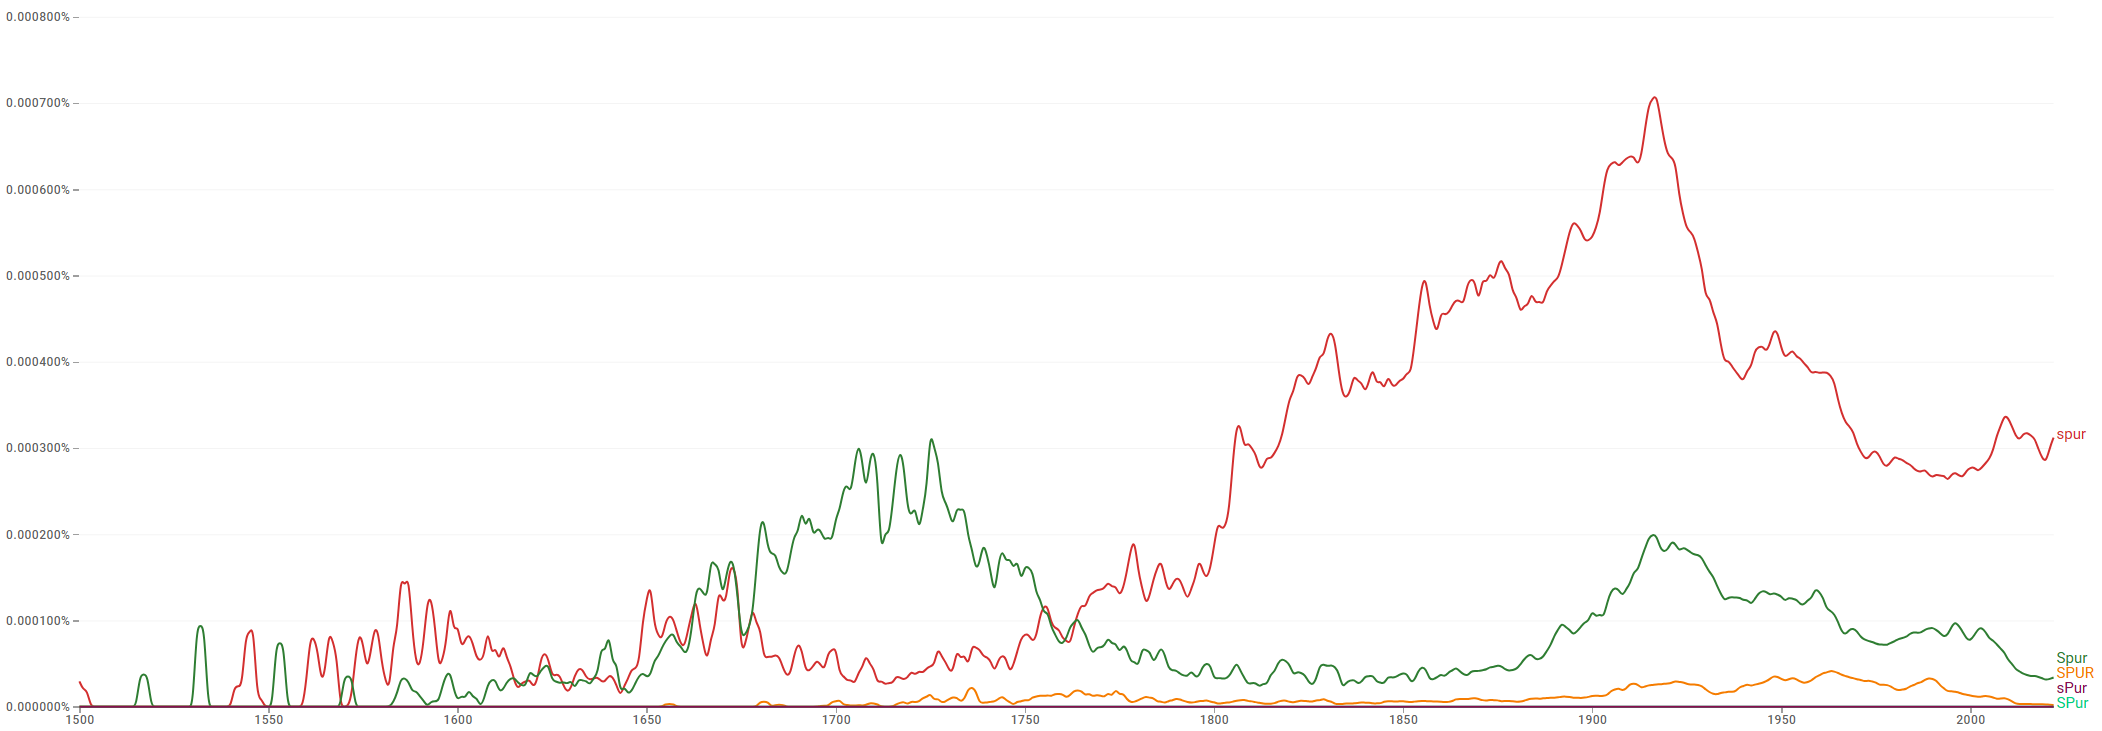
\includegraphics[width=1\linewidth]{Ngrams/SPUR.png}
    \caption{\href{https://books.google.com/ngrams/graph?content=SPUR&year_start=1500&year_end=2022&corpus=en&smoothing=1&case_insensitive=true}{SPUR no n-gram viewer entre 1500 e 2020}}
    \label{fig:SPUR}
\end{figure}

Há maneiras de obter dados nessas situações, utilizando termos alternativos que retornem resultados relevantes ao que se busca; adicionando \textit{n-grams} ao objeto de análise para proporcionar contexto, como "SPUR architecture", ou empregando o recurso de subtração para excluir resultados que desviem os valores, como "SPUR - SPUR Association". Embora essas soluções funcionem em muitos casos, elas não produzem resultados tão precisos quanto \textit{n-grams} únicos, o que pode gerar distorções nos resultados.

Outra limitação dessa ferramenta é que ela se restringe ao conteúdo disponível em livros, excluindo outros tipos de fontes que podem representar melhor a relevância de certos \textit{n-grams}, como artigos ou páginas da web. A frequência de \textit{n-grams} também pode não ser uma métrica muito precisa dependendo do objetivo da pesquisa, pois um livro pode usar o mesmo \textit{n-gram} várias vezes.

Um grande problema é que a frequência de uso de um \textit{n-gram} pode ser inflada se uma ou mais obras específicas mencionam o termo muitas vezes. Como a ferramenta calcula a frequência com base no número total de ocorrências em relação ao número total de palavras no corpus \cite{michel_quantitative_2011}, um único livro que utiliza um termo repetidamente pode aumentar desproporcionalmente a frequência de uso, dando uma impressão errônea da popularidade do termo. Portanto, mesmo que a frequência de uso de um termo seja maior do que a de outro, isso não indica diretamente seu nível de popularidade em comparação com outros termos.

Apesar destas desvantagens, este método é simples de ser executado, podendo fornecer uma rápida estimativa sobre a relevância do que esta sendo pesquisado. Além disto, há uma possibilidade de poder pesquisar diversos \textit{n-grams} ao mesmo tempo permite uma rápida comparação entre os períodos em que cada \textit{n-gram} foi mais usado.

\section{Análise em Bases Acadêmicas}

Para uma comparação direta da popularidade entre as arquiteturas de computadores, um passo adicional pode ser realizado utilizando ferramentas de busca de trabalhos acadêmicos. Este passo adicional oferece uma comparação da quantidade de trabalhos relacionados, em vez de apenas comparar a frequência de uso de termos específicos.

Esta análise pode ser combinada com a realizada no visualizador de Ngrams, proporcionando um entendimento mais amplo da relevância das arquiteturas. Enquanto o Ngram Viewer permite uma visualização da relevância ao longo do tempo, uma análise em uma base de dados oferece uma visão geral da relevância, pois os resultados são baseados em trabalhos publicados, não apenas no uso de termos. Isso possibilita uma comparação direta da relevância entre diferentes arquiteturas.

Para realizar esta análise, foram utilizadas duas bases de dados: o \href{https://scholar.google.com/}{Google Scholar} e o \href{https://www.periodicos.capes.gov.br/}{Periódicos Capes}. Cada uma dessas bases possui mecanismos de busca e artigos indexados diferentes, o que permite verificar tanto se as técnicas de pesquisa se aplicam para diferentes bases quanto realizar uma comparação para validação dos resultados. Adicionalmente, o Google Scholar permite pesquisas por patentes, aumentando o tipo de documentos incluídos na pesquisa.

\subsection{Vantagens e Desvantagens}

As pesquisas realizadas dentro das bases acadêmicas apresentam uma métrica de relevância mais precisa, isso por que ao invés de comparar a quantidade de vezes que um termo foi utilizado, estamos comparando a quantidade de trabalhos que apresentam este termo, eliminando problemas em situações onde poucos trabalhos citam o mesmo termo muitas vezes.

A filtragem dos termos também se torna bem mais simples, isso porque podemos combinar os nomes das arquiteturas com outros termos específicos removendo uma quantidade pequena de trabalhos relacionados. Isso se deve ao fato de que a combinação de termos pode diminuir a frequência de uso no geral, o que é ruim para uma análise nos Ngrams, porém dificilmente removerá trabalhos relevantes que devem citar estas combinações ao menos uma vez.

Embora as pesquisas em bases acadêmicas tenham suas vantagens, elas geralmente não oferecem uma forma fácil de análise temporal, limitando-se a filtros anuais. Isso é bastante restritivo em comparação com os Ngrams, que apresentam gráficos de fácil interpretação visual.

Além disso, algumas bases de dados podem não representar com precisão a totalidade dos trabalhos publicados. Por essa razão, é recomendada a utilização de mais de uma base para pesquisas deste tipo. O Google Scholar foi uma das bases escolhidas por apresentar uma quantidade massiva de trabalhos, o que pode atenuar essa desvantagem.

\section{Resultados}

\subsection{N-gram Viewer}

De todas arquiteturas pesquisadas, diversas não puderam ser pesquisadas com seus nomes diretamente devido aos problemas citados na Seção \ref{sec:ngram_pros_cons}, dentre dessas temos ARM, SPARC, MIPS, (Motorola)68000, Intel pré x86, x86, x64, SPUR, SOAR. As arquiteturas que não tiveram este problema incluem PowerPC, PA-RISC, RISC I, RISC II e RISC-V. 

\subsubsection{ARM}

Alguns dos nomes citados não representam uma só arquitetura, mas sim uma família de arquiteturas, como o ARM. Nestes casos, podemos usar diretamente o nome das versões das arquiteturas que existem dentro dessas arquiteturas, por exemplo, podemos analisar todas as versões de ARM existentes, que vão do ARMv1 até o ARMv8. As 3 primeiras versões do ARM não resultaram em nenhum valor, porém as subsequentes deram resultados significantes, com um aumento do uso a cada versão que foi lançada, que pode ser visto na Figura \ref{fig:NgramARM}.

\begin{figure}[H]
    \centering
    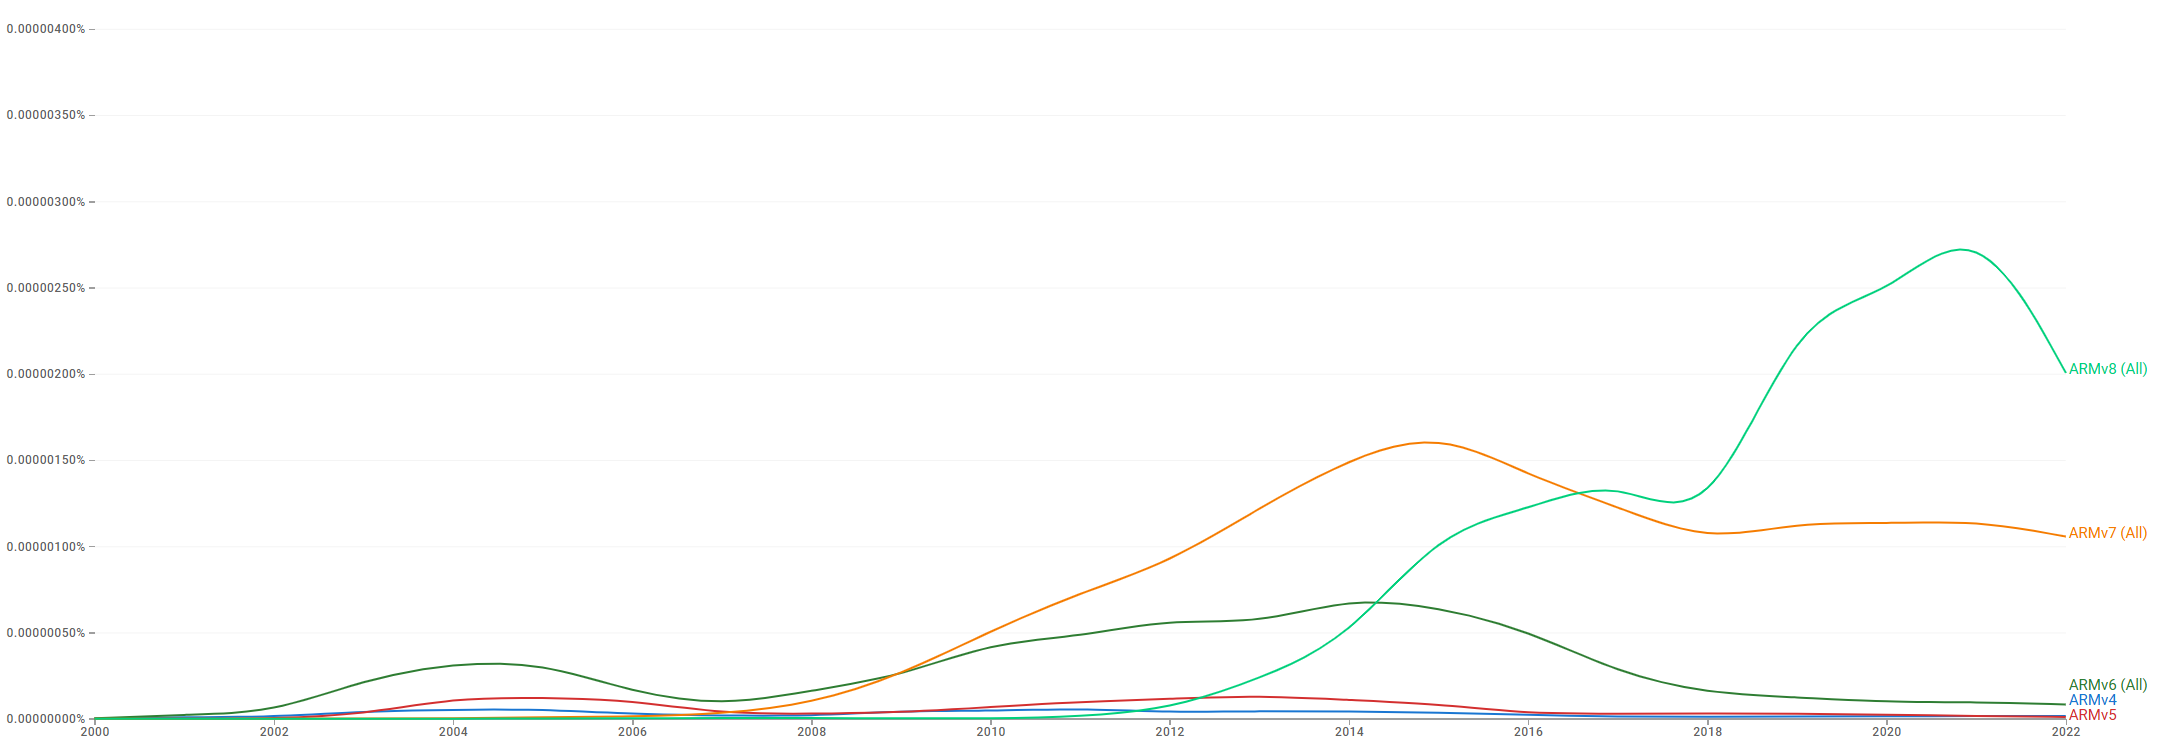
\includegraphics[width=1\linewidth]{Ngrams/ARM.png}
    \caption{\href{https://books.google.com/ngrams/graph?content=ARMv1\%2CARMv2\%2CARMv3\%2CARMv4\%2CARMv5\%2CARMv6\%2CARMv7\%2CARMv8&year_start=2000&year_end=2022&corpus=en&smoothing=1&case_insensitive=true}{Análise das versões do ARM}}
    \label{fig:NgramARM}
\end{figure}

\subsubsection{PA-RISC}

O PA-RISC é uma arquitetura que pode ser pesquisada diretamente pelo nome. No entanto, também foi testada a inclusão de arquiteturas individuais na análise. O resultado, presente na Figura \ref{fig:NgramPA-RISC}, apresentou valores baixos. Para comparação, foi adicionado o RISC I com um fator de 0,15x à sua frequência, considerando que o RISC I já possui uma frequência baixa, como será mostrado posteriormente.

\begin{figure}[h]
    \centering
    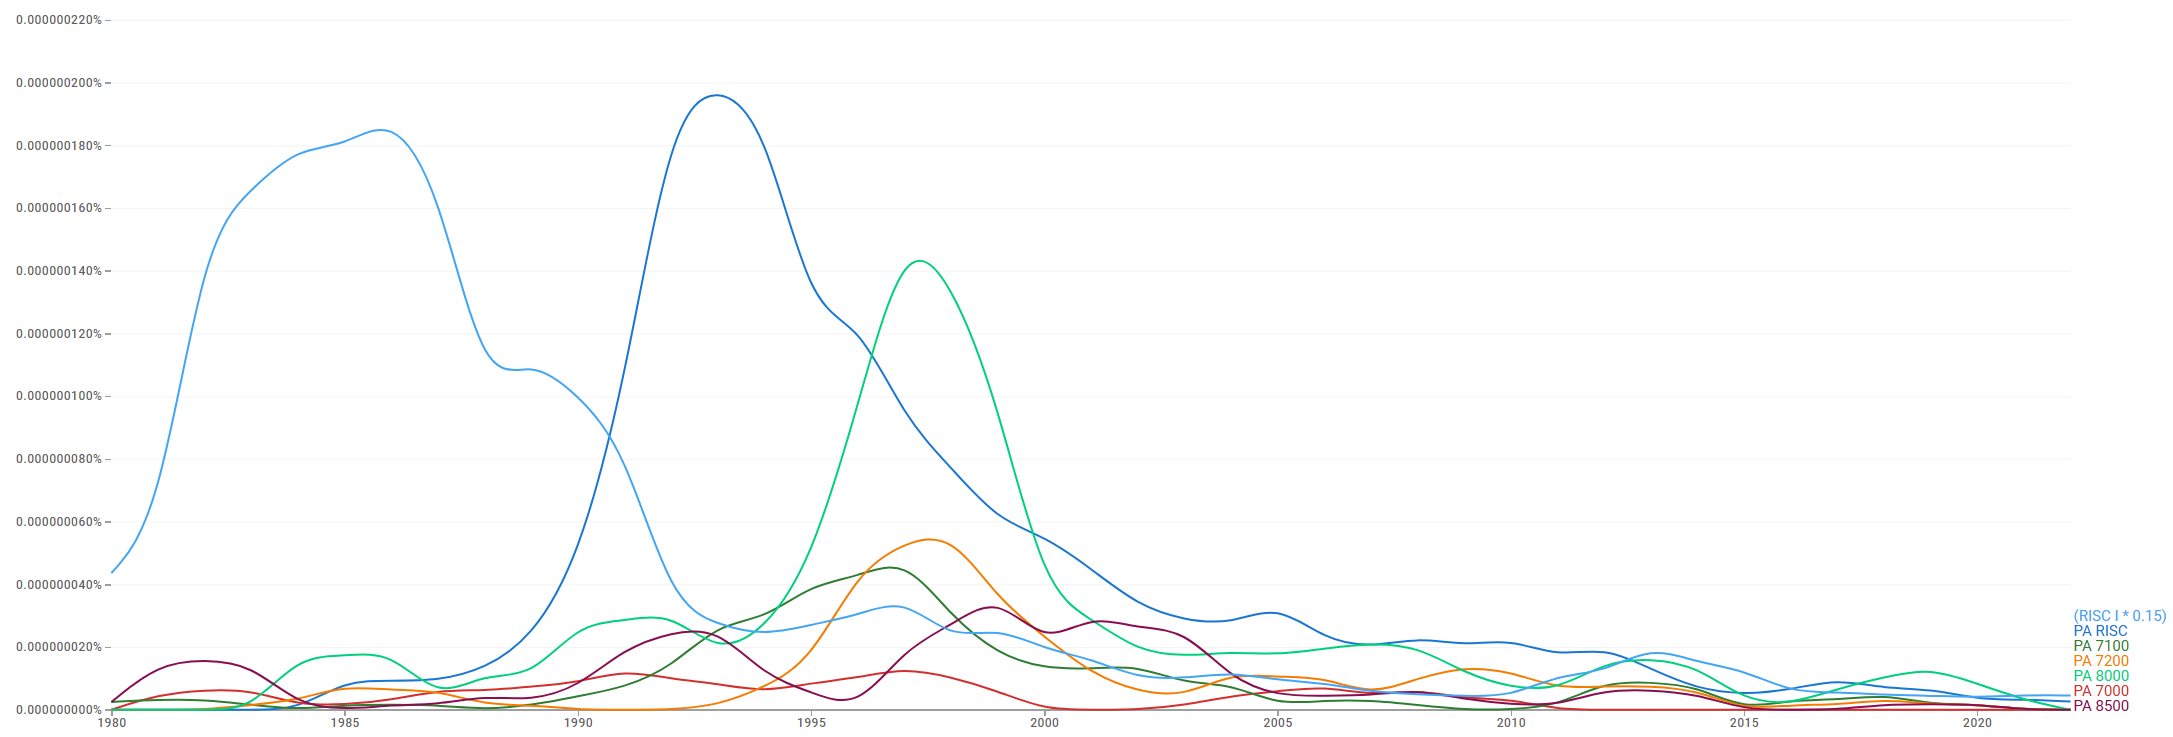
\includegraphics[width=1\linewidth]{Ngrams/PA_RISC.png}
    \caption{{\href{https://books.google.com/ngrams/graph?content=PA\%20RISC\%2CPA\%207000\%2CPA\%207100\%2CPA\%207200\%2CPA\%208000\%2CPA\%208500\%2C\%28RISC\%20I\%20\%2A\%200.15\%29&year_start=1980&year_end=2022&corpus=en&smoothing=1}{Análise do PA-RISC}}}
    \label{fig:NgramPA-RISC}
\end{figure}

\subsubsection{Berkeley RISC}

A Figura \ref{fig:NgramBerkeleyRISC} mostra uma comparação entre as arquiteturas Berkeley RISC. Exceto o RISC-V, essas arquiteturas surgiram como projetos acadêmicos e não possuem grande frequência de uso por não serem produtos comerciais. No entanto, ainda é importante analisar essas arquiteturas, especialmente as duas primeiras, que cunharam o termo RISC.

O RISC III e o RISC IV não eram chamados assim quando foram publicados. Em vez disso, foram chamados de SOAR (Smalltalk On A RISC) \cite{samples_soar_1985} e SPUR (Symbolic Processing Using RISCs) \cite{hill_spur_1985}, respectivamente. Apesar disso, o professor que orientou a criação dos RISCs originais, Patterson, considera esses como os RISCs III e IV \cite{patterson_risc-v_2016}.


\begin{figure}[h]
    \centering
    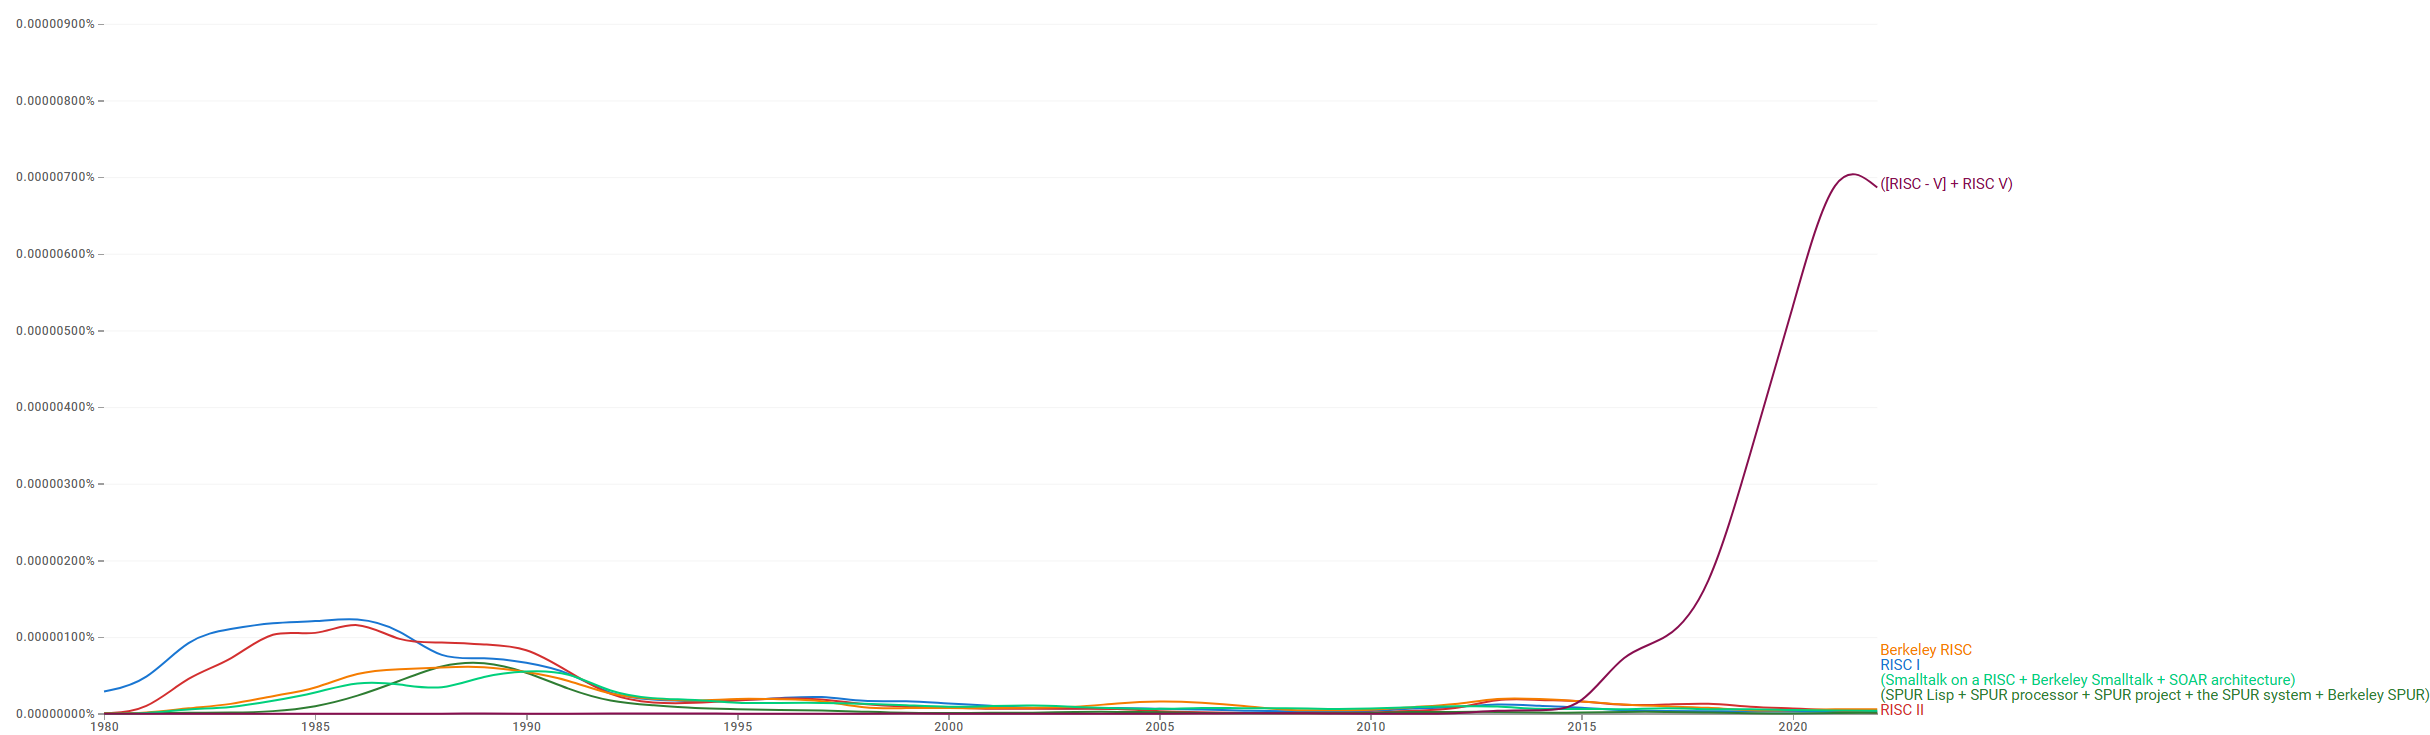
\includegraphics[width=1\linewidth]{Ngrams/Berkeley_RISC.png}
    \caption{\href{https://books.google.com/ngrams/graph?content=RISC\%20I\%2CRISC\%20II\%2CSPUR\%20Lisp\%20\%2B\%20SPUR\%20processor\%20\%2B\%20SPUR\%20project\%20\%2B\%20the\%20SPUR\%20system\%2BBerkeley\%20SPUR\%2CBerkeley\%20RISC\%2CSmalltalk\%20on\%20a\%20RISC\%20\%2B\%20Berkeley\%20Smalltalk\%20\%2B\%20SOAR\%20architecture\%2C\%5BRISC-V\%5D\%20\%2B\%20RISC\%20V&year_start=1980&year_end=2022&corpus=en&smoothing=1&case_insensitive=true}{Análise do Berkeley RISC}}
    \label{fig:NgramBerkeleyRISC}
\end{figure}

Tanto o SOAR quando o SPUR não puderam ser pesquisados diretamente, pois estes termos são utilizados em outros trabalhos não relacionados, e para solucionar isso, foram utilizados n-grams alternativos ou combinações que filtrassem resultados indesejados, e estes foram adicionados para obtenção de um gráfico único por arquitetura. Os resultados obtidos confirmam o fato de que as 3\degree e 4\degree versões não foram tão conhecidas como as duas primeiras, porém ainda há uma relevância significativa.

O RISC-V inicialmente também foi um projeto inicialmente desenvolvido na Universidade de Berkeley, porém este se tornou um padrão aberto da industria, comandado pela Fundação RISC-V\cite{patterson_risc-v_2016}, e como visto na Figura \ref{fig:NgramBerkeleyRISC}, esta versão tem se tornado bem mais popular que as suas anteriores.

\subsubsection{MIPS}

A arquitetura MIPS \cite{mips_tech_llc_mips32_2016}, assim como o ARM, foi pesquisada pelo nome de suas versões, conforme mostrado na Figura \ref{fig:NgramMIPS}. Embora tenha perdido popularidade nos últimos anos, ela possui características similares às do RISC.

Assim como a arquitetura Berkeley RISC, a arquitetura MIPS também surgiu de uma universidade e se tornou uma arquitetura comercial através da empresa MIPS Technologies, pouco após as primeiras publicações do RISC \cite{patterson_computer_1996}. Ela tem sido utilizada em algumas universidades para ensinar conceitos sobre arquitetura e organização de computadores \cite{vollmar_mips_2005}, mostrando o seu valor acadêmico.

Segundo \citeonline{turley_wait_2021}, a MIPS Technologies decidiu abandonar sua arquitetura tradicional e adotar a arquitetura RISC-V. Após passar por várias mudanças de propriedade e sair da falência, a empresa agora se concentra em desenvolver chips baseados na arquitetura RISC-V. Esta mudança marca o fim da linha para a família de CPUs MIPS e representa uma transformação completa no modelo de negócios da empresa, que antes se dedicava ao licenciamento de IP.

\begin{figure}[H]
    \centering
    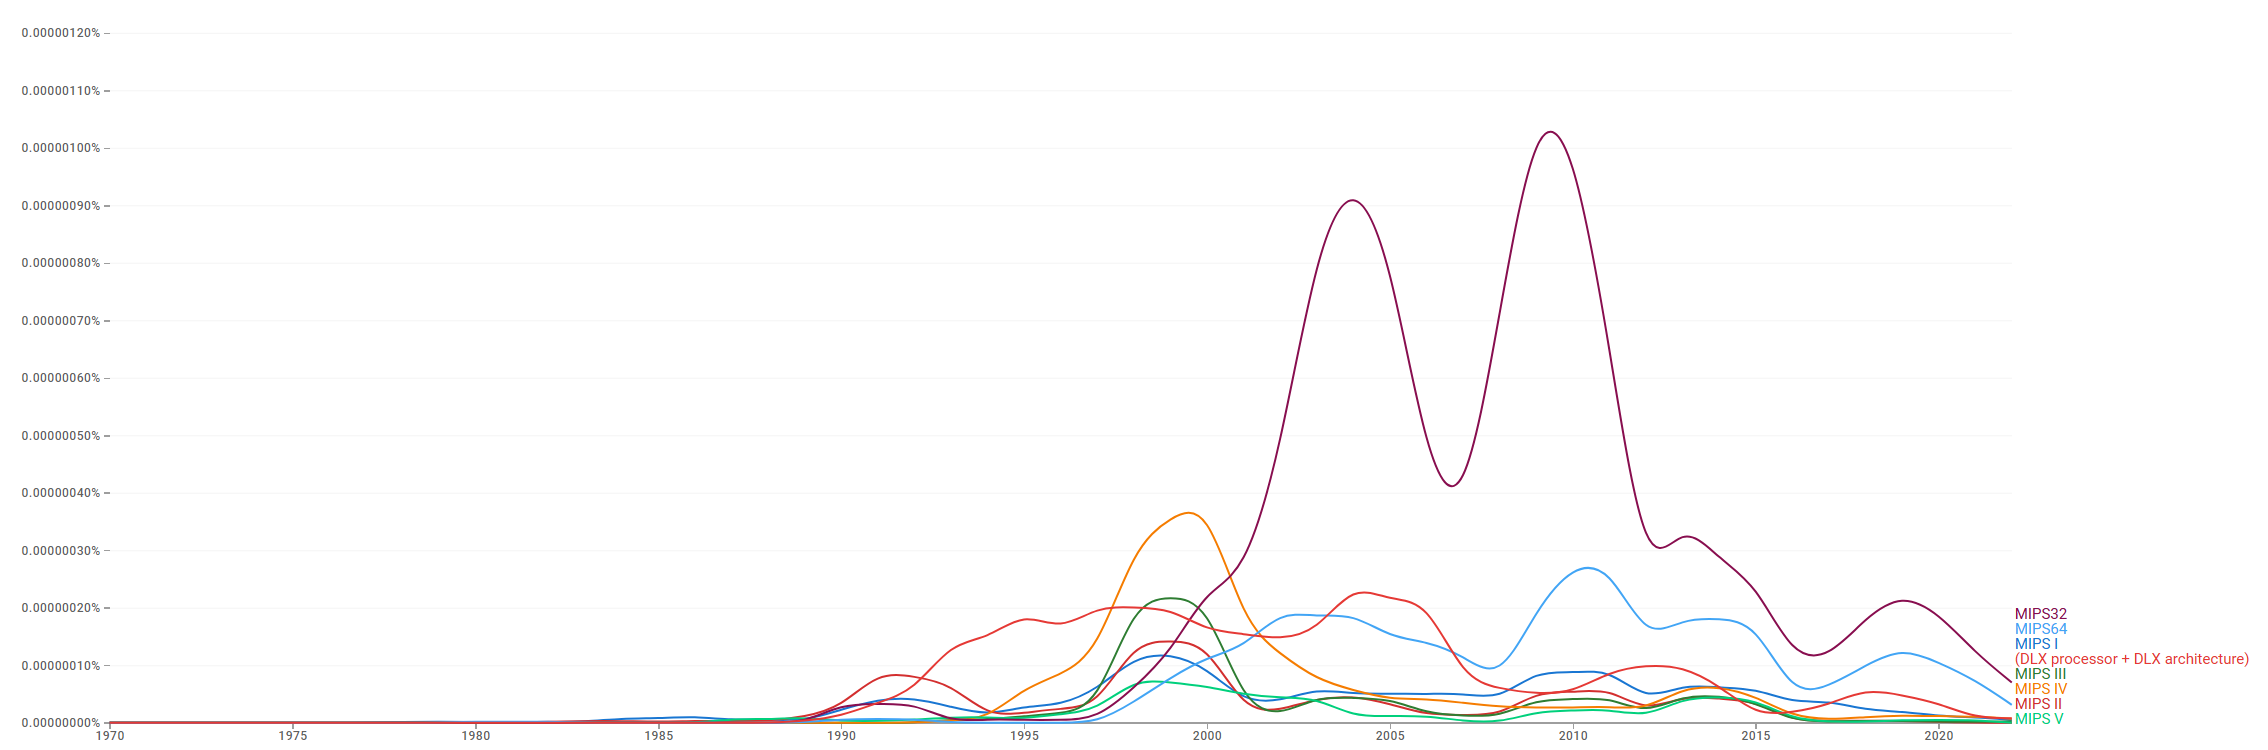
\includegraphics[width=1\linewidth]{Ngrams/MIPS_comparison.png}
    \caption{\href{https://books.google.com/ngrams/graph?content=MIPS\%20I\%2CMIPS\%20II\%2CMIPS\%20III\%2CMIPS\%20IV\%2CMIPS\%20V\%2CMIPS32\%2CMIPS64&year_start=1970&year_end=2022&corpus=en&smoothing=1&case_insensitive=false}{Análise do MIPS}}
    \label{fig:NgramMIPS}
\end{figure}

A DLX \cite{patterson_computer_1996}, uma arquitetura didática com diversas inspirações, sendo a principal delas a MIPS, foi incluída para comparação. Ela apresentou uma frequência de uso mais alta do que o esperado, mesmo que apenas nos casos onde acompanhava os termos "processor" e "architecture".

\subsubsection{Intel Pré x86}

As arquiteturas da Intel até o x86 foram analisadas, todas com o nome Intel junto do número. Apesar destas arquiteturas serem mais antigas em comparação a outras na pesquisa, elas ainda podem apresentar algum valor histórico ou características de interesse.

\begin{figure}[h]
    \centering
    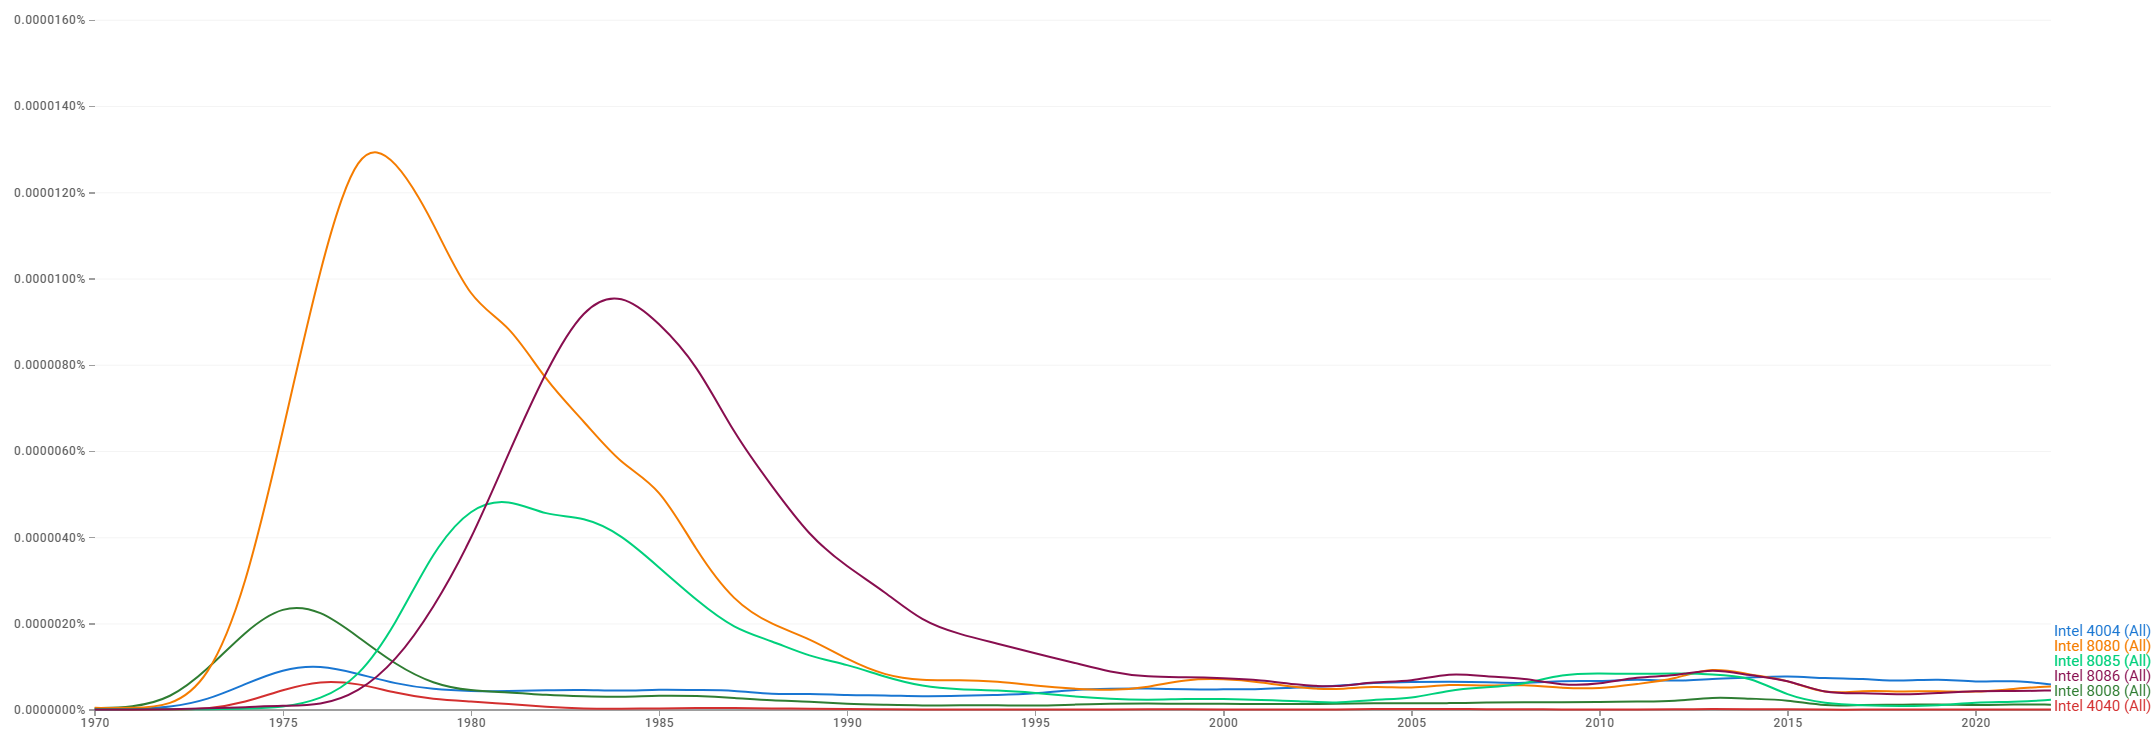
\includegraphics[width=1\linewidth]{Ngrams/Intel_pre_86.png}
    \caption{\href{https://books.google.com/ngrams/graph?content=Intel\%204004\%2CIntel\%204040\%2CIntel\%208008\%2CIntel\%208080\%2CIntel\%208085\%2CIntel\%208086&year_start=1970&year_end=2022&corpus=en&smoothing=1&case_insensitive=true}{Análise de arquiteturas Intel pré x86}}
    \label{fig:NgramIntelPre86}
\end{figure}

\subsubsection{Intel Pós x86}

As arquiteturas x86 e x64 são as mais comuns nos computadores domésticos atuais, sendo vendidas pelas empresas Intel e AMD, conforme visto em sites como \href{https://cpu.userbenchmark.com/}{UserBenchmark} e \href{https://store.steampowered.com/hwsurvey/processormfg/}{Steam Hardware Survey}. 

Alguns computadores possuem processadores ARM, mas esses ainda são a minoria fora do mercado de dispositivos móveis.

Uma análise sobre a frequência de uso dessas arquiteturas é um pouco difícil, pois os termos x86 e x64 trazem algum ruído por serem utilizados em outros contextos. Apesar disso, o resultado ainda é interessante, pois apesar da defasagem do x86 (32 bits) em favor do x64 (64 bits) nos últimos anos, sua frequência de uso na literatura tem se mantido bem mais alta que seu sucessor.

\begin{figure}[H]
    \centering
    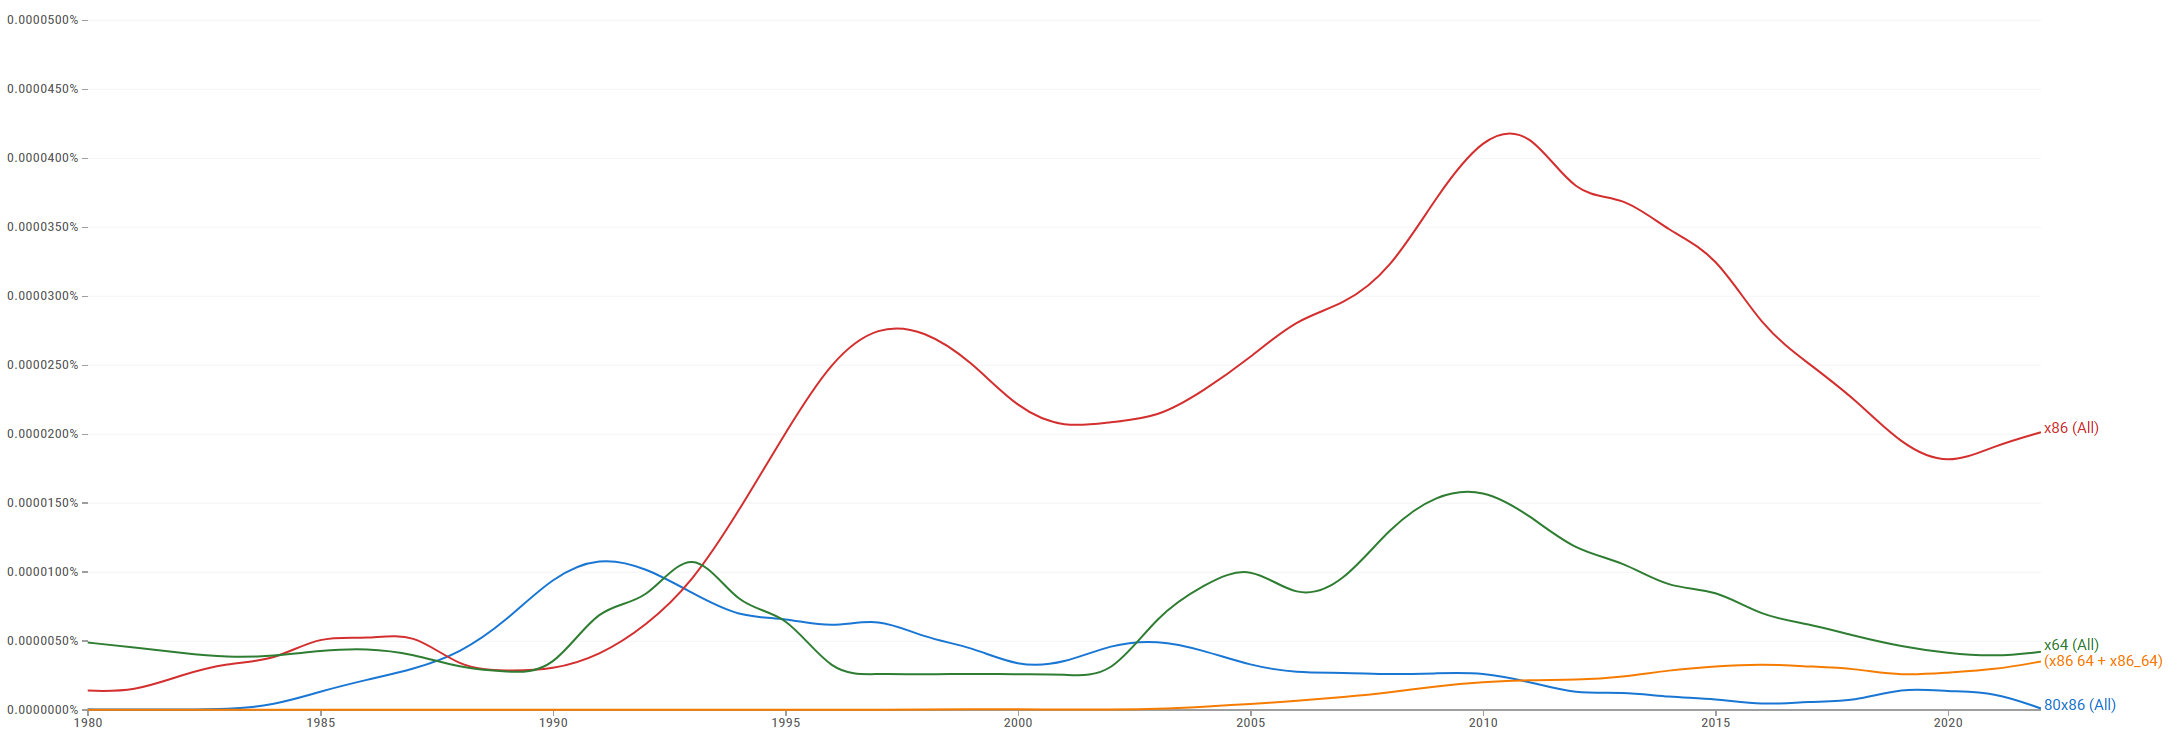
\includegraphics[width=1\linewidth]{Ngrams/x86_x64.png}
    \caption{\href{https://books.google.com/ngrams/graph?content=80x86\%2Cx86\%2Cx64\%2C\%28x86\%2064\%20\%2B\%20x86_64\%29&year_start=1980&year_end=2022&corpus=en&smoothing=1&case_insensitive=true}{Análise de arquiteturas pós x86}}
    \label{fig:NgramIntelPos86}
\end{figure}

\subsubsection{PowerPC}

A arquitetura PowerPC surgiu da aliança entre Apple, Motorola e IBM, e apesar de ter seu uso defasado durante anos, esta teve um grande pico de uso durante os anos 90 como visto na Figura \ref{fig:NgramPowerPC}, sendo utilizada até o início dos anos 2000.

\begin{figure}[h]
    \centering
    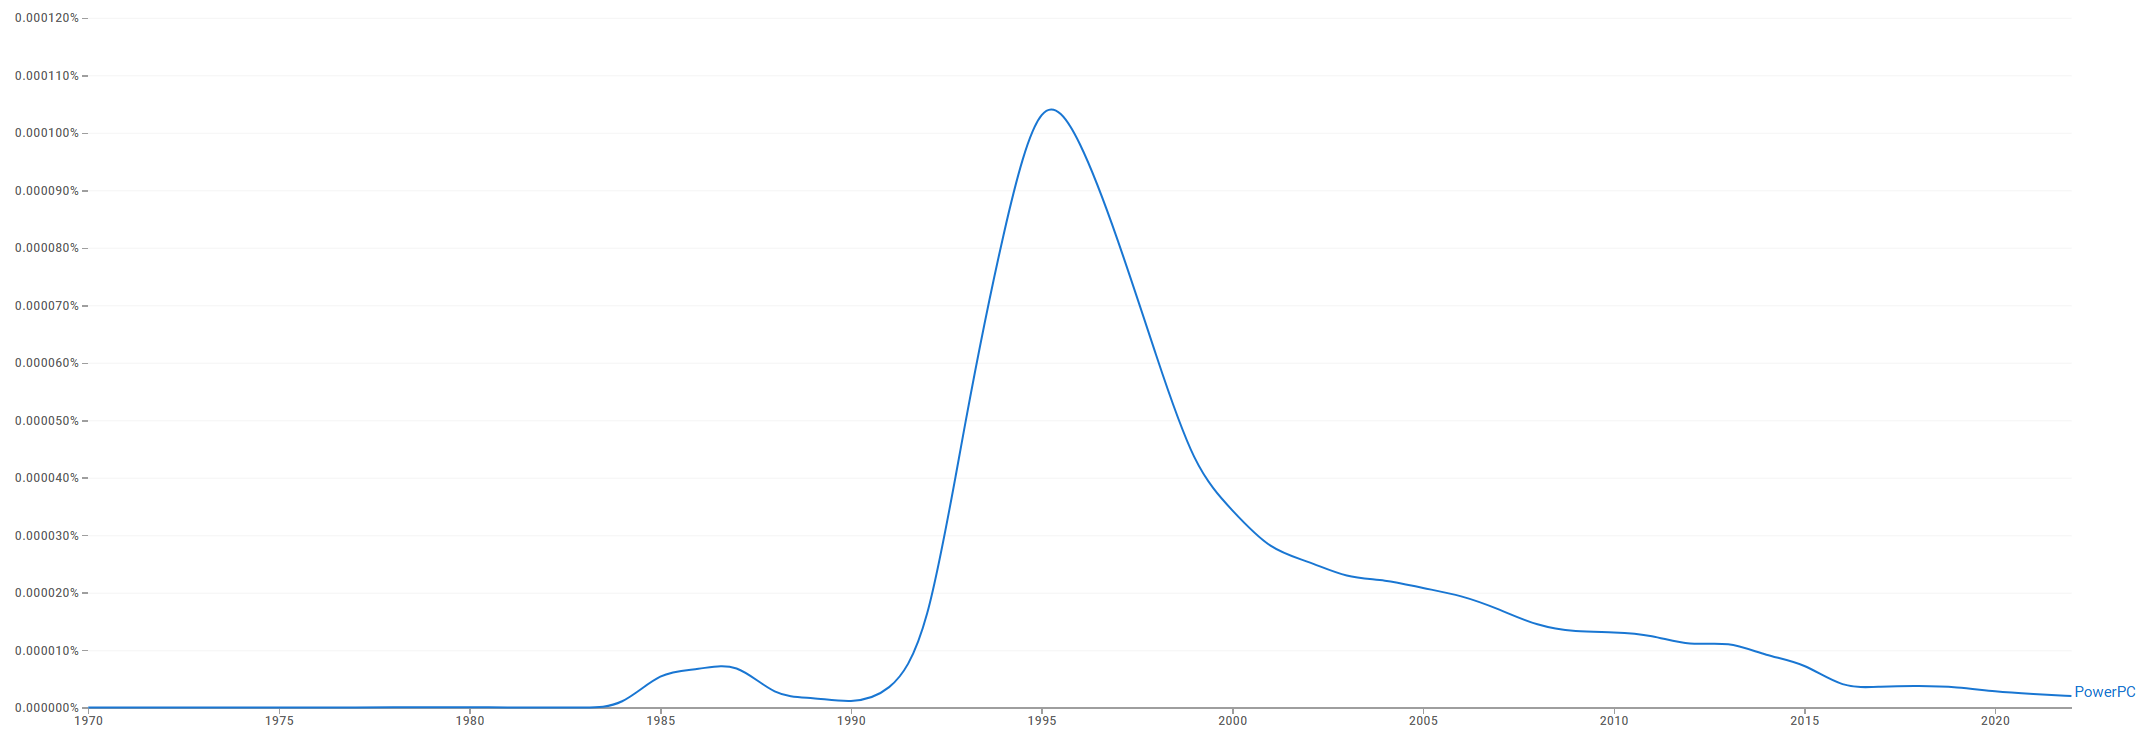
\includegraphics[width=1\linewidth]{Ngrams/PowerPC.png}
    \caption{\href{https://books.google.com/ngrams/graph?content=PowerPC&year_start=1970&year_end=2022&corpus=en&smoothing=1&case_insensitive=false}{Análise do PowerPC}}
    \label{fig:NgramPowerPC}
\end{figure}

\iffalse
\subsubsection{Motorola 68000}

A arquitetura Motorola 68000, assim como as arquiteturas Intel pré x86, não é utilizada frequentemente nos dias atuais, porém ainda 

\begin{figure}[h]
    \centering
    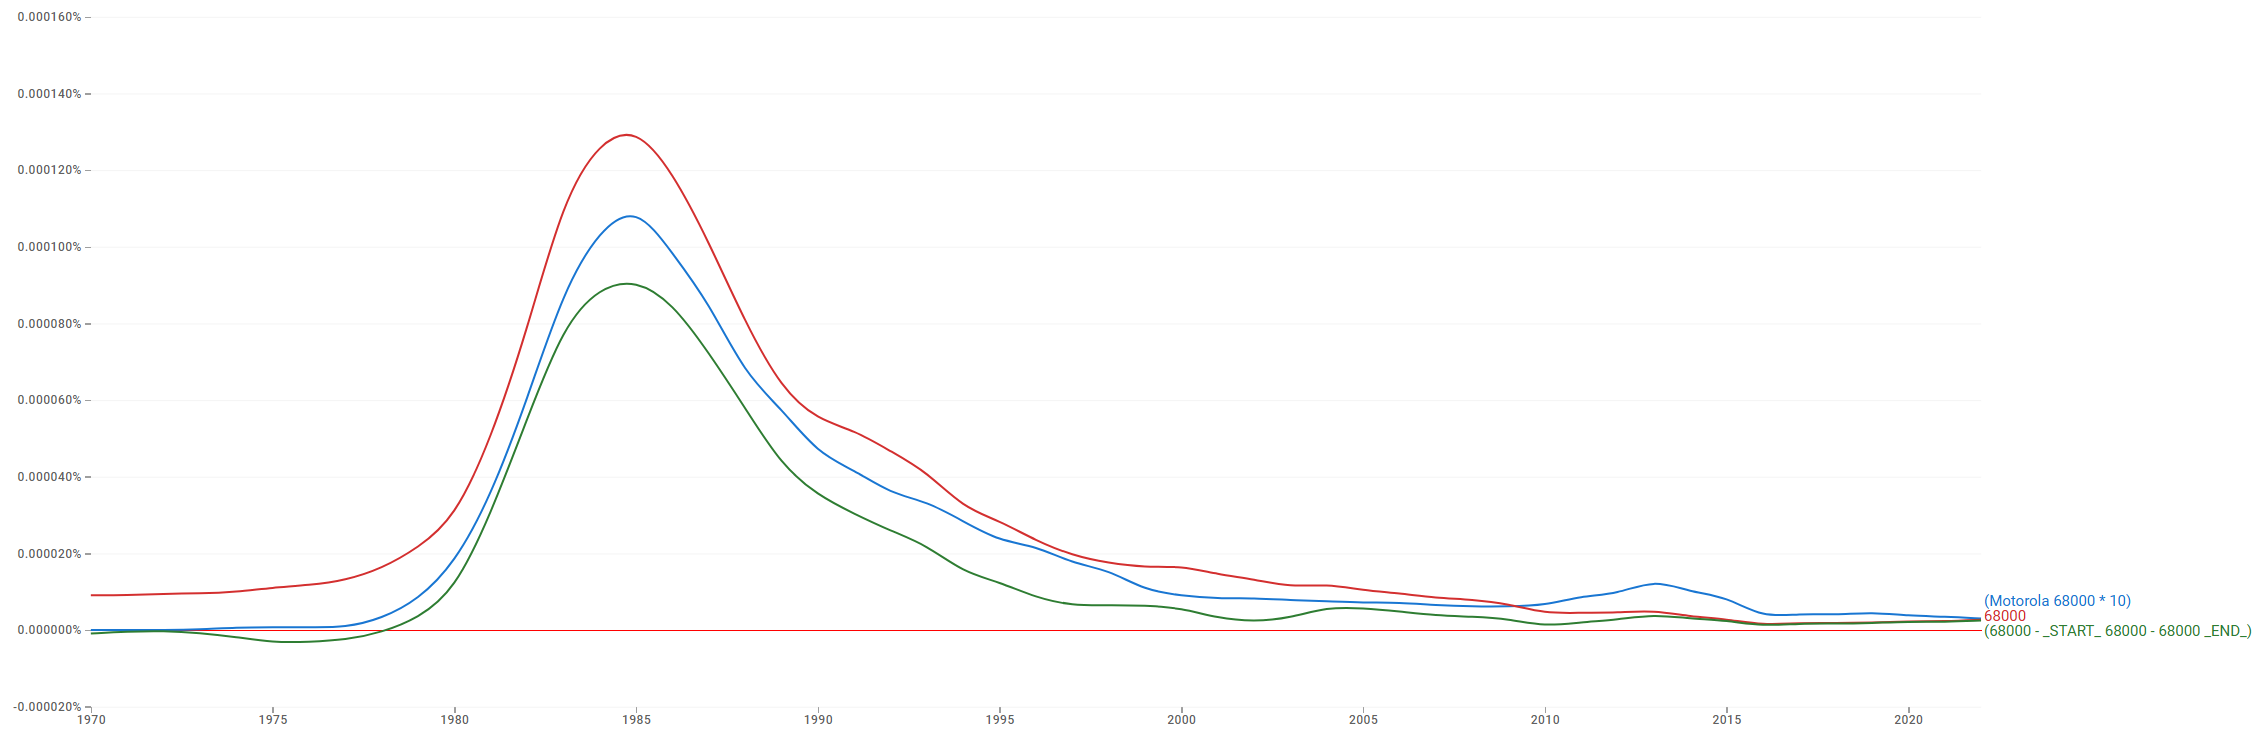
\includegraphics[width=1\linewidth]{Ngrams/Motorola68000.png}
    \caption{\href{https://books.google.com/ngrams/graph?content=(Motorola+68000*10),68000,(68000+-+_START_+68000+-++68000+_END_)&year_start=1970&year_end=2022&corpus=en&smoothing=1}{Análise do Motorola 68000}}
    \label{fig:Ngram68000}
\end{figure}
\fi

\subsubsection{SPARC}

A arquitetura SPARC, criada pela Sun Microsystems, é interessante por ser uma derivação direta do RISC-II \cite[p. 116]{patterson_computer_1996}. A pesquisa por este termo revelou uma frequência de uso anterior ao seu lançamento, como pode ser visto na Figura \ref{fig:NgramSPARC}. Esta figura também mostra o uso do recurso de \textit{wildcards}, que foi utilizado para identificar quais palavras acompanham o termo principal mais frequentemente, auxiliando na filtragem em alguns casos.

Embora seja útil em certas situações, no caso do SPARC, este recurso de \textit{wildcards} não foi tão eficaz, pois os termos mais comuns que acompanham o SPARC eram palavras conectivas, que não ofereciam o contexto do uso.

\begin{figure}[h]
    \centering
    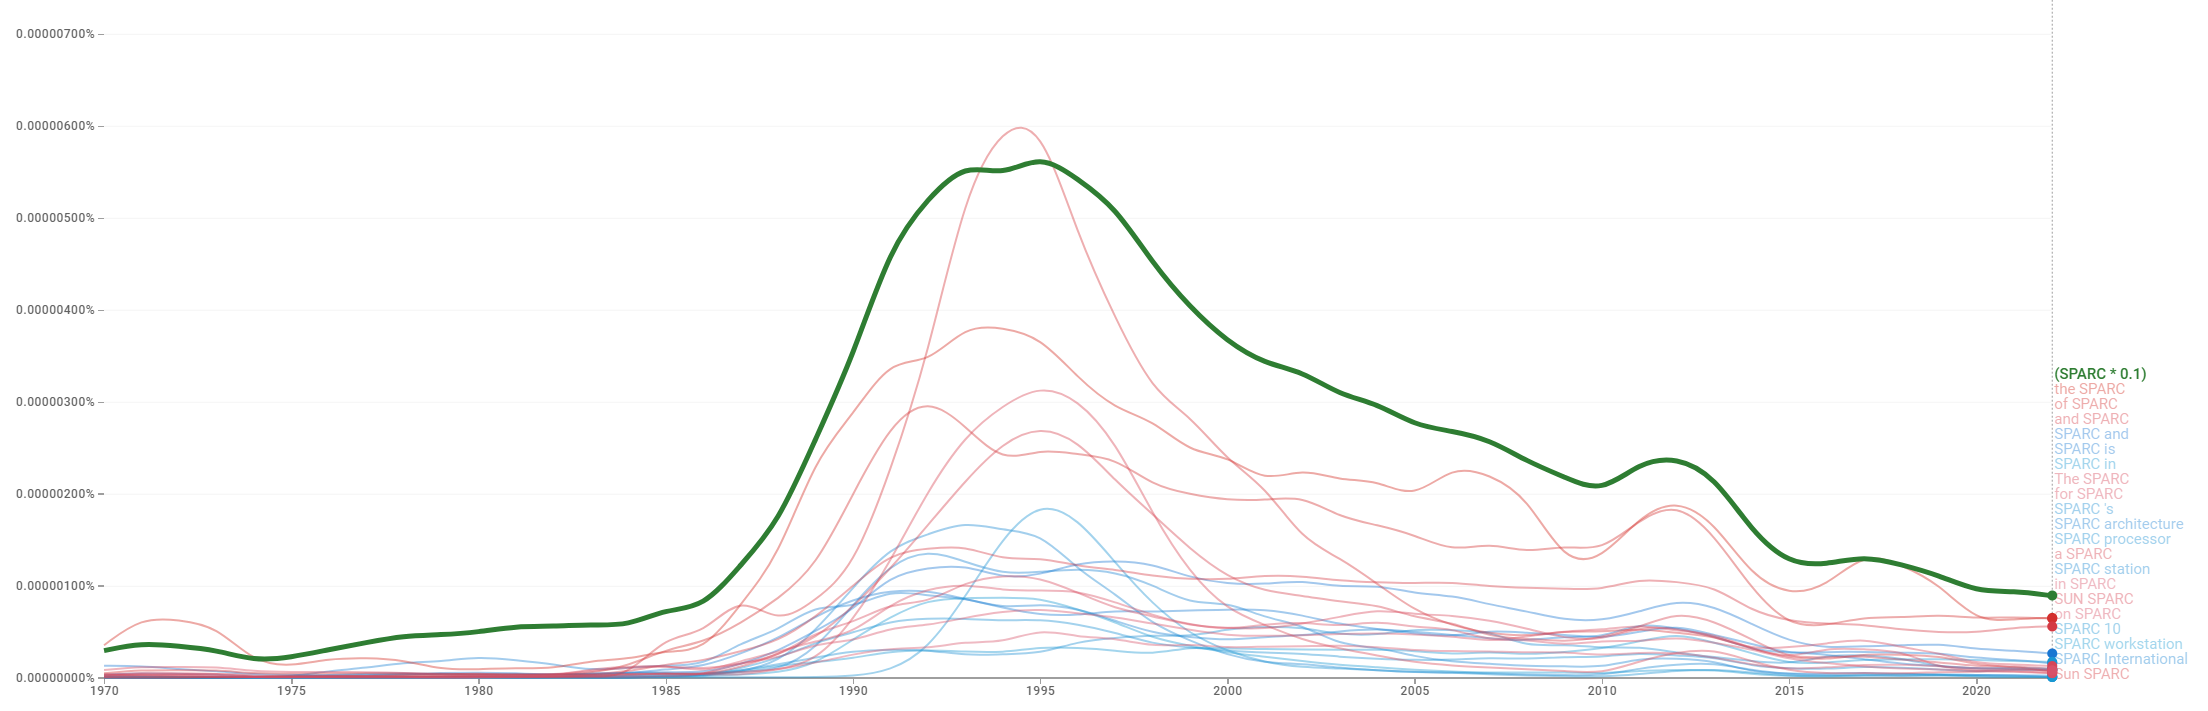
\includegraphics[width=1\linewidth]{Ngrams/SPARC_ALL.png}
    \caption{\href{https://books.google.com/ngrams/graph?content=SPARC *,* SPARC,(SPARC * 0.1)&year_start=1970&year_end=2022&corpus=en&smoothing=1}{Análise do SPARC}}
    \label{fig:NgramSPARC}
\end{figure}

O Ngram Viewer permite pesquisar as obras que utilizaram os termos, filtradas por época. Este recurso foi aproveitado para analisar os contextos em que o termo SPARC foi utilizado. Os contextos encontrados foram X3 SPARC, ANSI SPARC, SPARC DBMS e SPARC system, permitindo a subtração destes do termo SPARC. Para esta subtração, esses termos foram multiplicados por um fator de 10, o que reduziu a quantidade no gráfico para aproximadamente 0\% durante o período que a arquitetura SPARC ainda não existia.

Embora este processo introduza algumas imprecisões, o resultado, visto na Figura \ref{fig:NgramSPARC_Clean}, ainda possui relevância, indicando de forma mais clara o período em que o termo começou a se popularizar.

\begin{figure}[h]
    \centering
    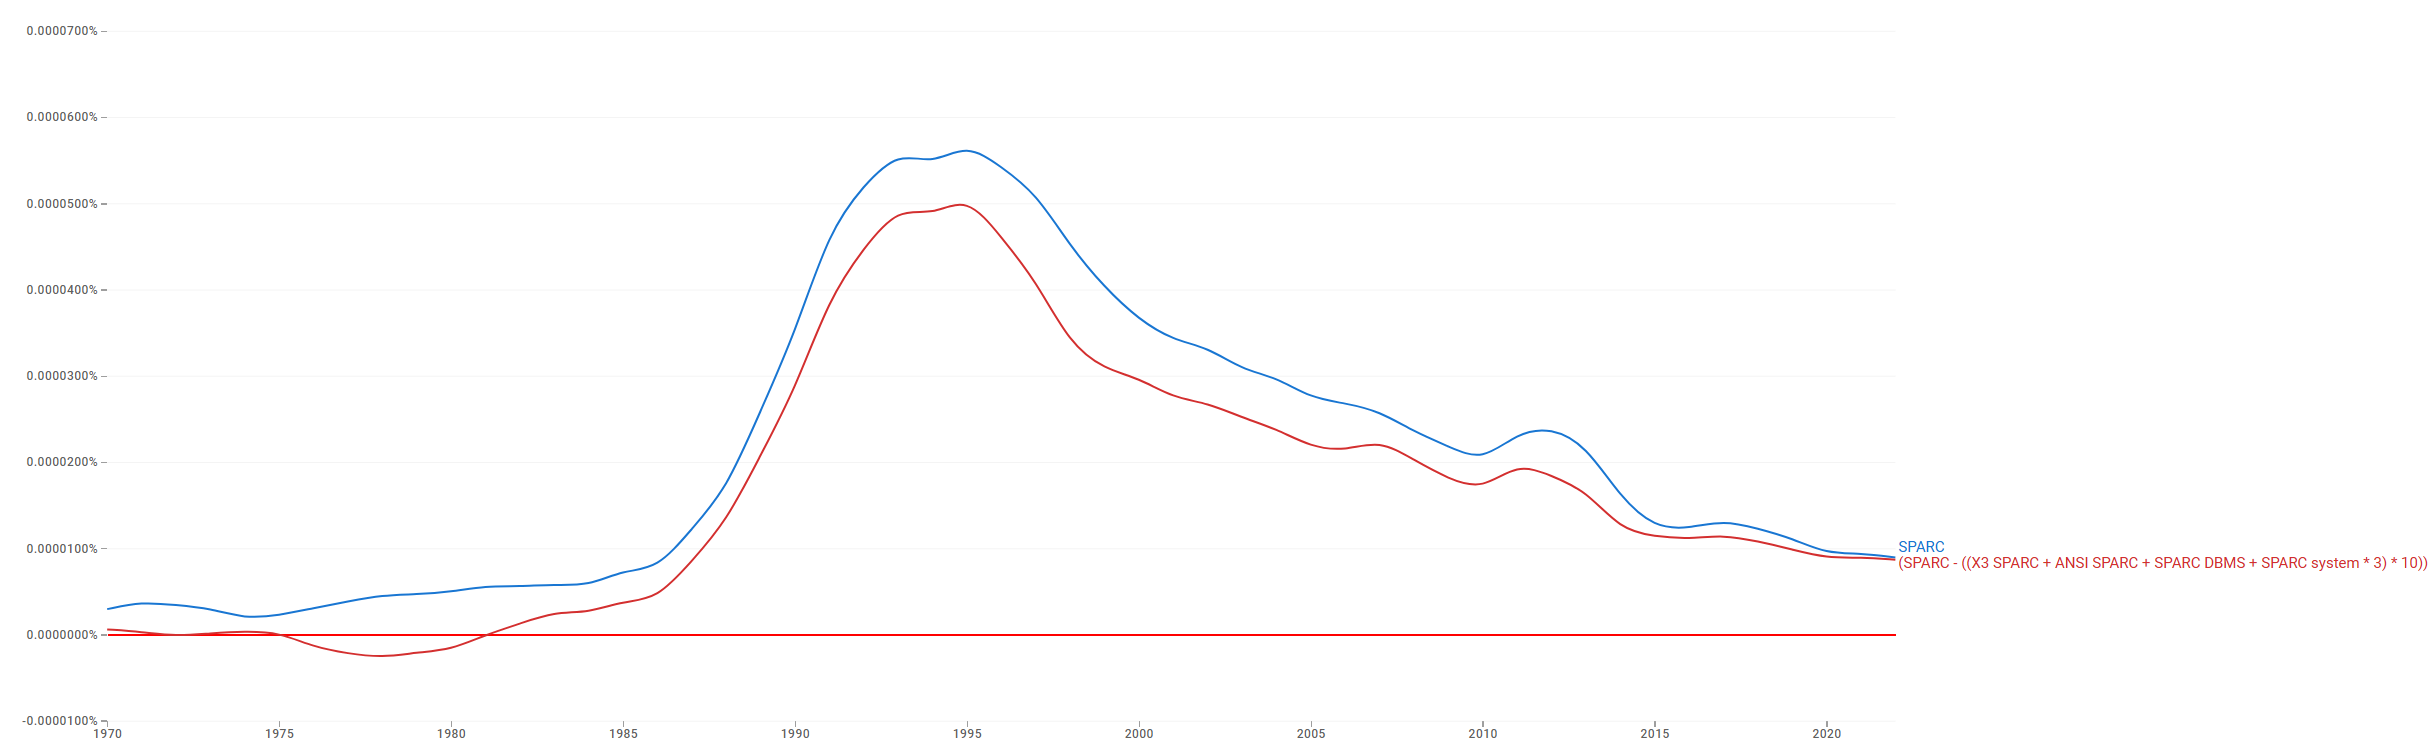
\includegraphics[width=1\linewidth]{Ngrams/SPARC_CLEAN.png}
    \caption{\href{https://books.google.com/ngrams/graph?content=SPARC,SPARC-((X3+SPARC+\%2B+ANSI+SPARC+\%2B+SPARC+DBMS+\%2B+SPARC+system+*+3)*10)&year_start=1970&year_end=2022&corpus=en&smoothing=1&case_insensitive=false}{Análise filtrada do SPARC}}
    \label{fig:NgramSPARC_Clean}
\end{figure}

\subsubsection{Análise Geral}

\begin{figure}[h]
    \centering
    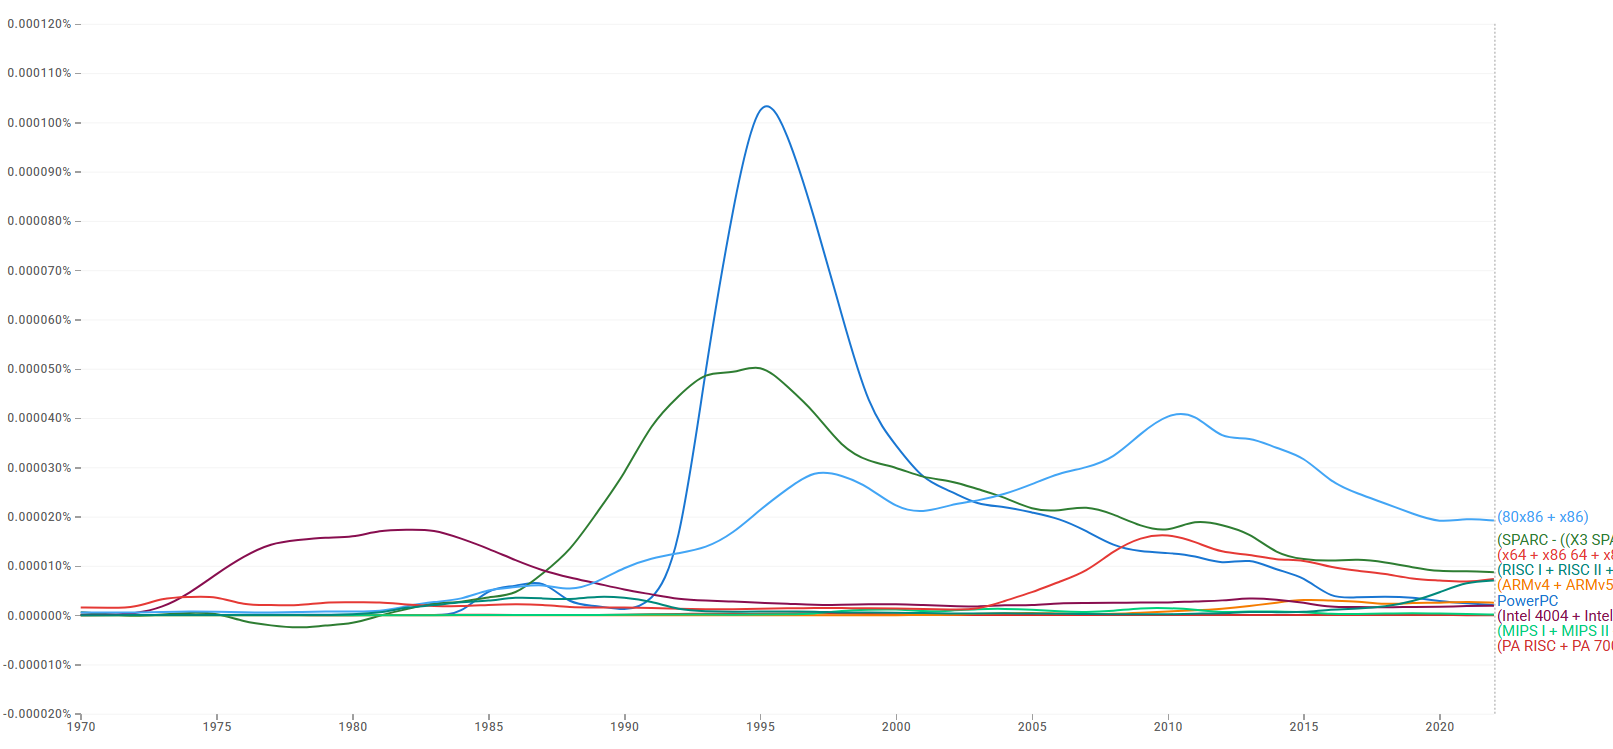
\includegraphics[width=1\linewidth]{Ngrams/full.png}
    \caption{\href{https://books.google.com/ngrams/graph?content=PowerPC,PA+RISC\%2BPA+7000\%2BPA+7100\%2BPA+7200\%2BPA+8000\%2BPA+8500,SPARC-((X3+SPARC+\%2B+ANSI+SPARC+\%2B+SPARC+DBMS+\%2B+SPARC+system+*+3)*10),ARMv4\%2BARMv5\%2BARMv6\%2BARMv7\%2BARMv8,MIPS+I\%2BMIPS+II\%2BMIPS+III\%2BMIPS+IV\%2BMIPS+V\%2BMIPS32\%2BMIPS64,Intel+4004\%2BIntel+4040\%2BIntel+8008\%2BIntel+8080\%2BIntel+8085\%2BIntel+8086,80x86\%2Bx86,(x64\%2Bx86+64+\%2B+x86_64),RISC+I\%2BRISC+II\%2BSPUR+Lisp\%2BSPUR+processor\%2BSPUR+project\%2Bthe+SPUR+system\%2BBerkeley+SPUR\%2BBerkeley+RISC\%2BSmalltalk+on+a+RISC\%2BBerkeley+Smalltalk\%2BSOAR+architecture\%2B[RISC-V]\%2BRISC+V&year_start=1970&year_end=2022&corpus=en&smoothing=1&case_insensitive=false}{Comparação entre todas as arquiteturas analisadas}}
    \label{fig:NgramFull}
\end{figure}

Ao analisar todos os \textit{n-grams} em conjunto (Figura \ref{fig:NgramFull}), observa-se que o PowerPC possui a maior frequência de uso, seguido pelas arquiteturas SPARC e x86. No entanto, exceto pela x86, essas arquiteturas têm perdido relevância ao longo dos anos, como indicado pela queda na frequência de uso dos termos na literatura. 

Para uma análise dos termos menos utilizados, foi criado um gráfico excluindo os \textit{n-grams} mais frequentes, presente na figura \ref{fig:NgramFull}. Ao analisar todas as arquiteturas, observa-se que o Berkeley RISC (atualmente RISC-V) destaca-se como a última arquitetura com um rápido aumento na frequência de uso, similar ao de outras arquiteturas que se tornaram populares em algum momento. Isso indica que ele pode ser um bom tema para estudos mais aprofundados.

Outra arquitetura interessante para estudo é a família ARM. Como mencionado anteriormente, o termo ARM não foi utilizado por certos fatores, o que diminui o seu gráfico de uso, porém, esta é uma arquitetura que esta presente em 99\% dos \textit{smartphones}, além de compor cerca de 50\% de todos os processadores utilizados atualmente\cite{arm_building_nodate}.


\begin{figure}
    \centering
    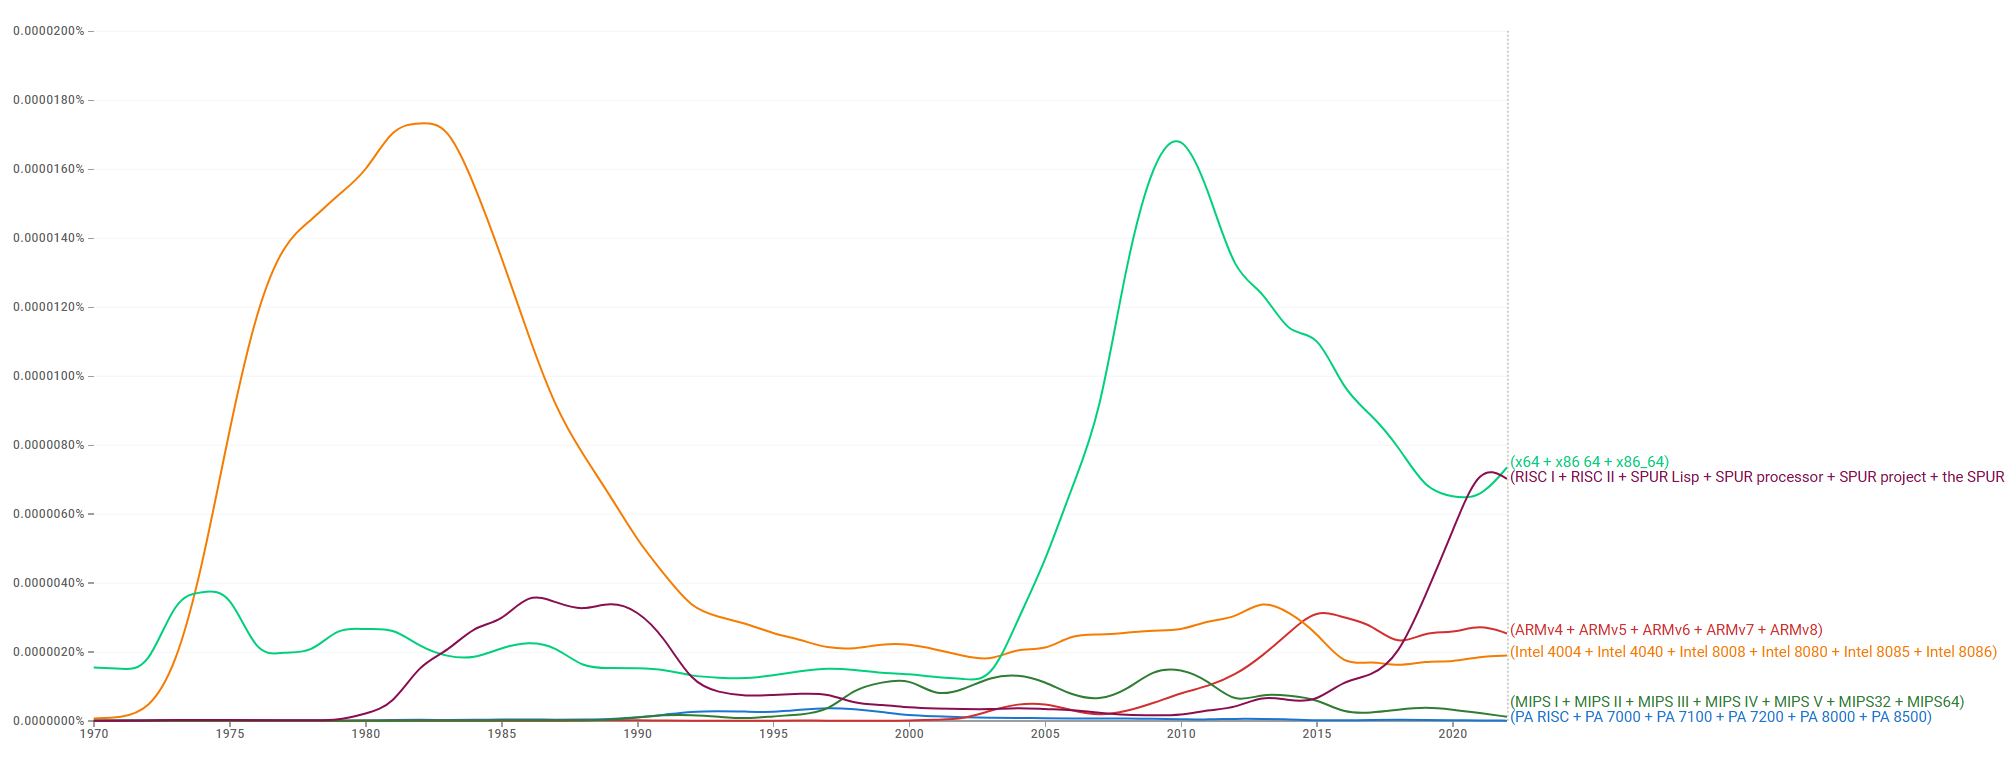
\includegraphics[width=1\linewidth]{Ngrams/Partial.png}
    \caption{\href{https://books.google.com/ngrams/graph?content=PA+RISC\%2BPA+7000\%2BPA+7100\%2BPA+7200\%2BPA+8000\%2BPA+8500,+ARMv4\%2BARMv5\%2BARMv6\%2BARMv7\%2BARMv8,+MIPS+I\%2BMIPS+II\%2BMIPS+III\%2BMIPS+IV\%2BMIPS+V\%2BMIPS32\%2BMIPS64,+Intel+4004\%2BIntel+4040\%2BIntel+8008\%2BIntel+8080\%2BIntel+8085\%2BIntel+8086,+(x64\%2Bx86+64+\%2B+x86_64),+RISC+I\%2BRISC+II\%2BSPUR+Lisp\%2BSPUR+processor\%2BSPUR+project\%2Bthe+SPUR+system\%2BBerkeley+SPUR\%2BBerkeley+RISC\%2BSmalltalk+on+a+RISC\%2BBerkeley+Smalltalk\%2BSOAR+architecture\%2B[RISC-V]\%2BRISC+V&year_start=1970&year_end=2022&corpus=en&smoothing=1}{Comparação entre as arquiteturas com menor frequência}}
    \label{fig:NgramParcial}
\end{figure}

\subsection{Análise em Bases Acadêmicas}

Foram realizadas oito pesquisas para cada arquitetura utilizando o Google Scholar: uma com o nome da arquitetura, denominada "Termo Individual", e sete combinando o nome da arquitetura com algum termo adicional para melhor filtragem dos resultados. A Tabela~\ref{fig:scholar} mostra os resultados dessas pesquisas, agrupados em quatro partes: o Termo Individual, os quatro termos com melhores resultados, a média e o desvio padrão entre eles, e, por fim, os três termos menos relevantes.

Os termos com os melhores resultados incluem palavras que geralmente são esperadas em trabalhos relacionados a arquiteturas computacionais, como \textit{architecture} (arquitetura), \textit{processor} (processador), \textit{instruction set} (conjunto de instruções) e \textit{computing} (computação). Ao realizar as buscas, o nome da arquitetura foi mantido entre aspas para correspondências exatas, porém o termo adicional não, o que permitiu uma filtragem mais ampla. Por exemplo, ao invés de aceitar apenas resultados com o termo \textit{computing}, o Google Scholar também aceita resultados com o termo \textit{computer} (computador), que, apesar de ser uma palavra diferente, ainda se encaixa no contexto desejado.

Os valores dos melhores resultados têm seu desempenho e precisão medidos pela média e desvio padrão. Espera-se que esta média represente um resultado mais filtrado em comparação ao Termo Individual, que pode estar presente em situações não relacionadas ao que se deseja, similar ao que ocorreu com as buscas no Ngram Viewer. Esta média pode indicar a relevância real de um resultado em comparação aos outros. O desvio padrão, por outro lado, é uma métrica do quanto esses termos podem afetar a quantidade de resultados, e, neste caso, quanto menor, melhor, indicando que, independentemente do termo escolhido, a quantidade de resultados é sempre consistente.

\begin{table}[h]
    \centering
    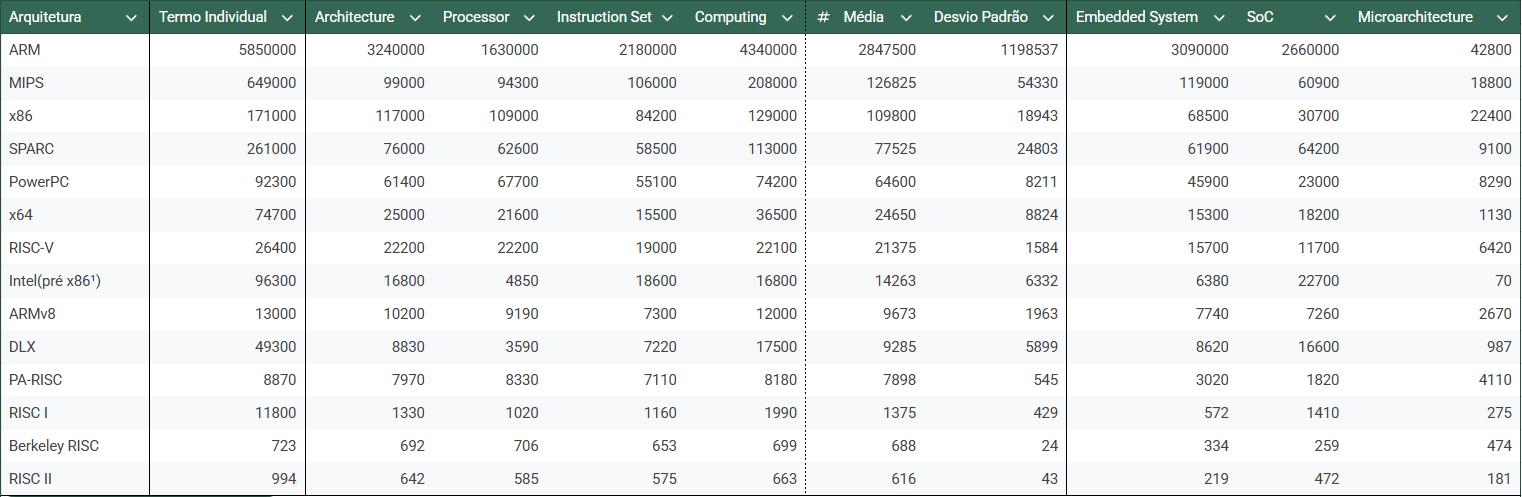
\includegraphics[width=1\linewidth]{BaseDeDados/scholar.png}
    \caption{Quantidade de Resultados de Pesquisa no Google Scholar}
    \label{fig:scholar}
\end{table}

Entre os termos menos relevantes, dois são mais focados em aplicações específicas - \textit{embedded system} (sistema embarcado) e \textit{SoC} (Sistema em um Chip) - e um é menos utilizado - \textit{micro architecture} (microarquitetura) - que acaba sendo um subconjunto de arquitetura. Estes termos retornaram menos resultados no geral, mostrando que eles podem não ser ideais para pesquisas gerais sobre arquiteturas. Isso fica claro observando a Tabela~\ref{fig:scholarProx}, que mostra que a porcentagem de resultados encontrados em relação ao nome da arquitetura isolado é bem menor em comparação ao resto dos termos, com o valor máximo de 65,6\%.

A Tabela~\ref{fig:scholarProx} complementa os resultados apresentados na Tabela~\ref{fig:scholar}, convertendo a quantidade de resultados em percentuais relativos aos resultados obtidos utilizando apenas o Termo Individual. Com exceção do desvio padrão, observa-se que uma menor porcentagem indica resultados menos satisfatórios ao utilizar somente o nome da arquitetura, pois isso sugere que o nome está sendo empregado em contextos não relacionados aos termos adicionais. Além disso, esta tabela facilita a análise do desvio padrão, uma vez que a utilização de percentuais permite uma comparação mais precisa entre as diferentes arquiteturas.

Ambas tabelas foram ordenadas a partir da média, o que resulta em diferentes perspectivas. Na primeira, quanto maior a média de resultados com o parâmetro adicional, mais popular e relevante podemos considerar esta arquitetura. Por outro lado na Tabela~\ref{fig:scholarProx}, como dito anteriormente, quanto menor o percentual, menos o nome da arquitetura é utilizado no contexto de computação. O RISC~I por exemplo foi encontrado em diversos contextos médicos que não se encaixam com o desejado. 

\begin{table}[h]
    \centering
    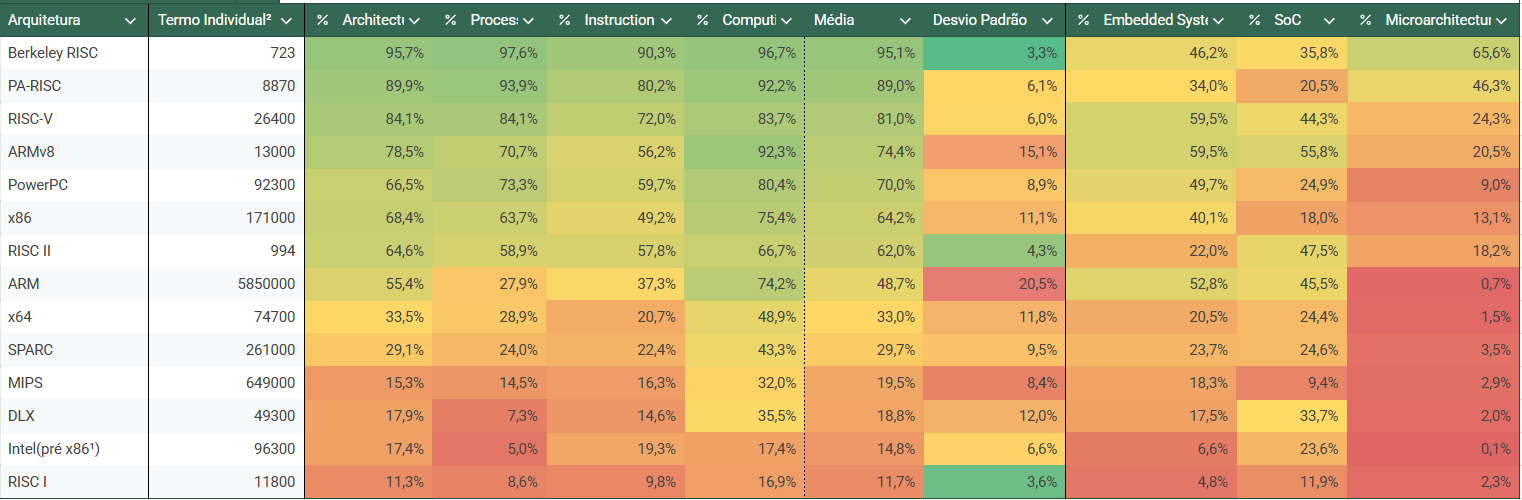
\includegraphics[width=1\linewidth]{BaseDeDados/scholarProx.png}
    \caption{Comparação de Proximidade dos Resultados de Pesquisa no Google Scholar}
    \label{fig:scholarProx}
\end{table}

\begin{table}[H]
    \centering
    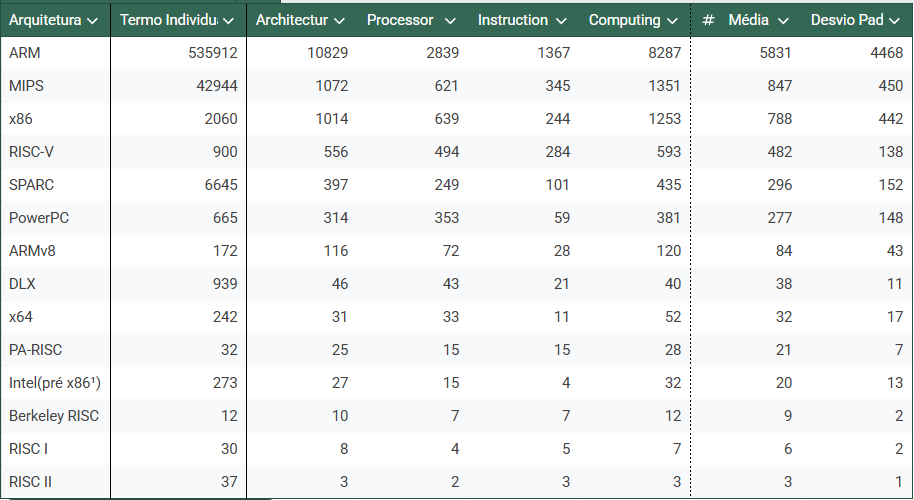
\includegraphics[width=1\linewidth]{BaseDeDados/capes.png}
    \caption{Quantidade de Resultados de Pesquisa no Periódicos Capes}
    \label{fig:capes}
\end{table}

Observa-se nas Tabelas \ref{fig:scholarProx} e \ref{fig:capesProx} que os nomes mais distintos apresentaram os maiores percentuais consistentemente nas duas bases de dados analisadas. Entre esses nomes, destacam-se Berkeley RISC, PA-RISC, RISC-V, ARMv8, PowerPC e x86. Como mostrado na Tabela \ref{fig:diff} Estes tiveram uma variação percentual entre 20,1\% e 26\% por arquitetura entre bases acadêmicas além de um desvio padrão entre 9,3\% e 17,1\% menor na base de dados Periódicos CAPES, indicando resultados mais consistentes ao utilizar diferentes termos adicionais.

\begin{table}[H]
    \centering
    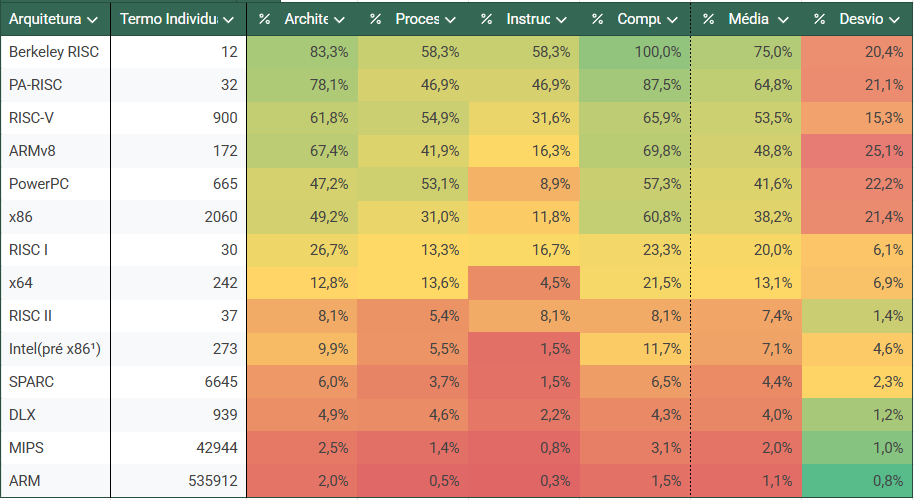
\includegraphics[width=1\linewidth]{BaseDeDados/capesProx.png}
    \caption{Comparação de Proximidade dos Resultados de Pesquisa no Periódicos Capes}
    \label{fig:capesProx}
\end{table}

\begin{table}[H]
    \centering
    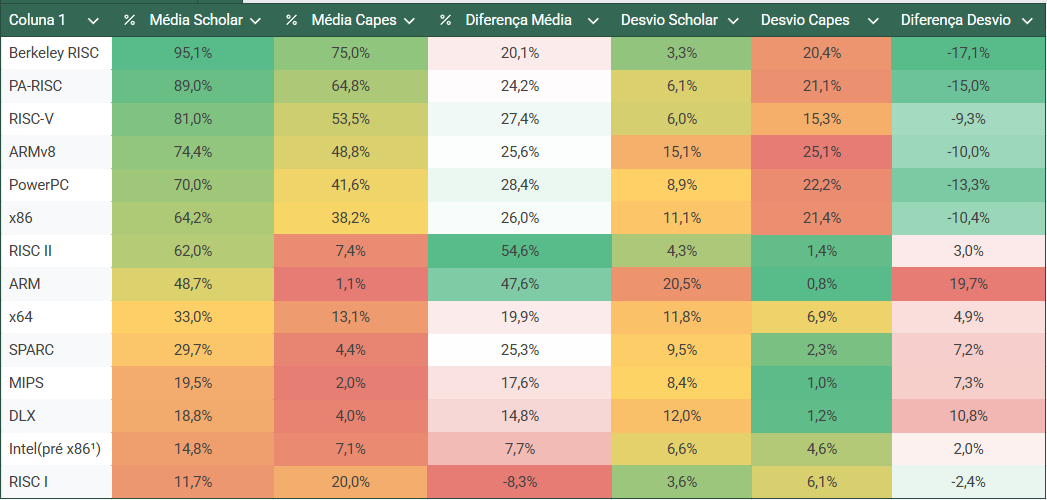
\includegraphics[width=1\linewidth]{BaseDeDados/diff.png}
    \caption{Diferença da média e do desvio padrão entre as bases acadêmicas.}
    \label{fig:diff}
\end{table}

Por outro lado, as arquiteturas com as menores médias percentuais apresentaram uma variação muito mais ampla, com RISC II e ARM retornando, respectivamente, aproximadamente 54,6\% e 47,6\% de resultados a menos na base de dados Periódicos CAPES. De modo geral, o desvio padrão dessas arquiteturas no CAPES foi menor, o que pode ser atribuído à alta discrepância na média de resultados relevantes entre as bases de dados.
\subsection{Análise Geral}

Ao comparar os resultados obtidos nas pesquisas com os resultados dos Ngrams, podemos corroborar a precisão de certos achados e corrigir outros. A arquitetura ARM, apesar de sua relevância significativa na atualidade, não apresentou altos valores nos Ngrams devido à filtragem realizada, que considerou apenas os resultados das arquiteturas individuais. Nas pesquisas, foram utilizados tanto os termos "ARM" quanto "ARMv8", uma das versões do ARM. O nome genérico ARM, como esperado, possuía uma grande quantidade de ruído nos resultados, o que foi parcialmente mitigado pela filtragem com termos adicionais, embora não o suficiente para removê-lo da primeira posição.

Por outro lado, a versão individual "ARMv8", assim como nos Ngrams, não apresentou tantos resultados quanto o nome genérico da arquitetura. No entanto, obteve uma alta média percentual de resultados relevantes, demonstrando que, apesar de ser uma filtragem rigorosa, ela aumenta significativamente a precisão dos resultados.

De forma semelhante ao observado no Ngram Viewer, a arquitetura x86 destacou-se com um dos maiores resultados, enquanto sua sucessora, x64, posicionou-se duas posições abaixo no Google Scholar, confirmando sua relevância. Em contraste, a arquitetura SPARC, que possuía uma frequência mais alta no Ngram Viewer, ficou abaixo do x86. Este dado sugere duas possibilidades: ou o nome x86 foi utilizado com menos frequência em comparação ao SPARC, apesar da maior quantidade de documentos, ou a filtragem no Ngram Viewer não foi suficientemente eficaz. Independentemente disso, o fato de ambas as arquiteturas estarem próximas nas duas métricas confirma um certo nível de consistência nos dados.

Apesar da arquitetura MIPS ter alcançado valores elevados, pesquisas pelas suas versões individuais resultaram em valores baixos, em torno de 2000 resultados, similar à frequência dos seus Ngrams. Isso pode ser devido ao fato de que o termo MIPS pode se referir a "Million Instructions Per Second" (Milhões de Instruções por Segundo), uma métrica usada para medir a velocidade de um processador. Logo, mesmo que a quantidade de resultados seja alta, há uma chance de que parte desses resultados contenha ruído dentro da própria área de computação.

O PowerPC, como esperado, foi uma das arquiteturas com menos ruído e, como indicado pelos Ngrams, a quantidade de resultados foi relativamente alta, embora ainda menor que a do x86 e do SPARC. Os Ngrams mostram que, apesar do PowerPC possuir o maior pico de todos, este não durou muito tempo, com um período de pouco menos de uma década, o que pode explicar sua posição nas tabelas.

O RISC-V obteve o terceiro maior percentual de resultados relevantes. Apesar de ser uma arquitetura recente (2010), retornou uma quantidade significativa de resultados, não muito distante do x64, que surgiu mais de uma década antes (1999). O rápido aumento da frequência de uso exibido nos Ngrams e a quantidade de resultados indicam que o RISC-V pode ser um forte competidor contra outras arquiteturas recentes.

A arquitetura PA-RISC apresentou mais resultados do que o esperado, considerando os dados dos Ngrams, além de ter o segundo maior percentual de fontes relevantes em ambas as bases acadêmicas. Apesar disso, ainda não possui grande popularidade, sendo uma arquitetura comercial. Para comparação, o PA-RISC ficou atrás da arquitetura DLX, que é puramente acadêmica.

As arquiteturas RISC originais, apesar de sua importância e influência nas arquiteturas RISC atuais, resultaram em uma quantidade ínfima de resultados em comparação com as outras, ficando nas três últimas posições na tabela. O termo Berkeley RISC retornou o maior percentual de resultados relevantes entre todas as arquiteturas, contrastando com as arquiteturas RISC~I e RISC~II, que apresentaram grande ruído devido à utilização desses termos em pesquisas médicas recentes.


% ---
% Finaliza a parte no bookmark do PDF, para que se inicie o bookmark na raiz
% ---
\bookmarksetup{startatroot}% 
% ---

% ---
% Conclusão
% ---
\clearpage
\section*{Considerações finais}
\addcontentsline{toc}{section}{Considerações finais}

Embora os métodos de pesquisa aplicados neste estudo tenham fornecido resultados satisfatórios para trabalhos onde a precisão não é crucial, em contextos que exigem alta precisão, seria necessário um exame mais detalhado. A filtragem no Google Ngram Viewer deve ser realizada com maior cautela, analisando minuciosamente os termos que causam ruído nos resultados. Esse método funciona bem para análises de relevância ao longo do tempo, mostrando os períodos em que determinados termos foram mais utilizados.

A aplicação conjunta de ambos os métodos de pesquisa ajudou a mitigar suas limitações, pois cada método complementou as informações que o outro não apresentava. Enquanto o Visualizador de Ngrams não oferece uma métrica eficiente de relevância geral entre termos, as pesquisas em bases acadêmicas não permitem uma análise temporal de relevância de forma fácil. Com ambos os métodos, podemos determinar se uma arquitetura ainda é relevante e qual é seu nível de relevância em comparação com outras.

Para pesquisas futuras, recomenda-se o desenvolvimento de métodos de filtragem mais robustos para melhorar a precisão dos resultados. Além disso, é essencial realizar uma pesquisa mais minuciosa que envolva as diversas arquiteturas individuais, em vez de termos genéricos como "ARM" em todos métodos envolvidos. Esta abordagem mais detalhada não foi adotada neste estudo devido a limitações de tempo e à falta de necessidade deste nível de detalhamento no contexto atual.

% ----------------------------------------------------------
% ELEMENTOS PÓS-TEXTUAIS
% ----------------------------------------------------------
\postextual

% ---
% Título e resumo em língua estrangeira
% ---

% \twocolumn[    		% INICIO DE ARTIGO EM DUAS COLUNAS

% titulo em inglês
\titulo{A Webbibliometry About the Relevance of Computer Architectures}
\emptythanks
\maketitle

% resumo em português
\renewcommand{\resumoname}{Abstract}
\begin{resumoumacoluna}
 \begin{otherlanguage*}{english}
   This article explores the educational application of computational architectures by conducting a bibliometric analysis to evaluate the relevance of RISC architectures within the broader context of computing systems. Leveraging tools such as the Google Books Ngram Viewer and academic databases like Google Scholar and CAPES Journals, the study identifies trends and patterns in the evolution and adoption of computational architectures. Key findings include the chronological prominence of RISC-based designs and their influence on modern architectures such as RISC-V. The research combines historical usage data with an evaluation of academic publication trends, offering insights into the enduring significance of these architectures for educational and technological advancements.
   \vspace{\onelineskip}
 
   \noindent
   \textbf{Key-words}: computational architectures, RISC, bibliometric analysis, Ngram Viewer, academic relevance.
 \end{otherlanguage*}  
\end{resumoumacoluna}

% ]  				% FIM DE ARTIGO EM DUAS COLUNAS
% ---

% ----------------------------------------------------------
% Referências bibliográficas
% ----------------------------------------------------------
\bibliography{references}


\begin{apendicesenv}
\end{apendicesenv}
\begin{anexosenv}
\end{anexosenv}
\end{document}
